\PassOptionsToPackage{final}{graphicx}
\documentclass[usepdftitle=false,xcolor=table,9pt]{beamer}

%\usepackage{fontspec}
%\defaultfontfeatures{Mapping=tex-text}
%\usepackage{xunicode}
%\usepackage{xltxtra}
%
%\usepackage{xeCJK}
%\setCJKmainfont{MS Mincho}

\usepackage[T1]{fontenc}


\usepackage{etex}
\usepackage{tkz-graph}
%\newif\ifmydraft
%% \mydrafttrue
%\mydraftfalse
%% \usepackage{pgfpages}


% \newcommand{\WIP}{\framesubtitle{Draft version of this slide}}
\newcommand{\WIP}{}
\newcommand{\cha}{\textnormal{char}}
\tikzset{
   invisible/.style={opacity=0,text opacity=0},
   visible on/.style={alt=#1{}{invisible}},
   alt/.code args={<#1>#2#3}{\alt<#1>{\pgfkeysalso{#2}}{\pgfkeysalso{#3}}},
    beameralert/.style={alt={<#1>{fill=red!30,rounded corners}{}},anchor=base},
    BeamerAlert/.style={alt={#1{fill=red!30,rounded corners}{}},anchor=base}
}
\newcommand<>{\tikzMe}[1]{% previously: \def\tikzMe<#1>#2{…
 \tikz[baseline]\node[BeamerAlert={#2},anchor=base] {#1};
}


\AtBeginSection[]{\begin{frame}<beamer>\frametitle{Table of contents}\tableofcontents[currentsection]\end{frame}}
\AtBeginSubsection[]{\begin{frame}<beamer>\frametitle{Table of contents}\tableofcontents[currentsubsection]\end{frame}}

\mode<presentation> {
  \usetheme{Malmoe}
  % ou autre ...
  % \useinnertheme{rounded}
  \usecolortheme{rose}
  \usecolortheme{seahorse}
  % \useoutertheme{infolines}
  \setbeamercovered{invisible}
  \setbeamertemplate{navigation symbols}{%
    \usebeamerfont{footline}%
    \usebeamercolor[fg]{footline}%
    % \usebeamercolor[bg]{normal text}%
    %\insertframenumber%
  }
  \setbeamertemplate{headline}{}
  \setbeamertemplate{footline}[frame number]{}

  \setbeamertemplate{section in toc}[sections numbered]
  \setbeamertemplate{subsection in toc}{\leavevmode\leftskip=1.5em{\usebeamercolor[fg]{structure}\usebeamertemplate{itemize subitem}{}}\hspace{0.5em}\usebeamercolor{normal text}\usebeamerfont{subsection in toc}\normalsize\inserttocsubsection\par}

  % \setbeamerfont{itemize subitem}{size=\large}
  % \setbeamertemplate{itemize subbody begin}{\normalsize}
}

\setbeamersize{text margin left=0.3cm}
\setbeamersize{text margin right=0.3cm}



% \usepackage{setspace}% http://ctan.org/pkg/setspace
% \let\oldframetitle\frametitle% Store old \frametitle in \oldframetitle
% \renewcommand{\frametitle}[1]{% Redefine \frametitle
% \oldframetitle{#1}\setstretch{1.6}}
\addtobeamertemplate{frametitle}{\vspace*{-0cm}}{\vspace*{-0.4cm}}

\setbeamerfont{itemize/enumerate subbody}{size=\normalsize}

\newcommand{\greenframe}{\setbeamercolor{frametitle}{parent=block body example, fg=black}}

\newenvironment{alertbulletenv}{\only{\setbeamercolor{local structure}{fg=myred}}}{}

\usepackage[utf8]{inputenc}

% \usepackage{tgheros}

% \usepackage[scaled]{helvet}
% \usepackage{mathptmx}
\usepackage[tt=false]{libertine}
\usepackage[scaled=0.77]{beramono}

\usepackage{stmaryrd}


% \usepackage{libertinus}

% \usepackage[slantedGreek]{cmbright}

% \DeclareMathAlphabet{\mathcal}{OMS}{cmsy}{m}{n}

% \usepackage{sansmathaccent}
% \usepackage{lmodern}
\usepackage[T1]{fontenc}
% Or autre. Notez que le codage et la fonte doivent être assortis. Si T1
% ne paraît pas très esthétique, essayer d'effacer la ligne contenant fontenc.

% \usepackage{translator}
\uselanguage{English}
\languagepath{English}

\usepackage[british]{babel}
\usepackage{csquotes}

\usepackage{ifthenx}
\usepackage{xstring}

\usepackage[draft]{fixme}
\fxsetup{author={T},envlayout={color},%
  layout={footnote,marginclue},theme=color}
\newcommand{\ifxnote}[1]{\fxnote[inline,nomarginclue,nofootnote]{#1}}
\newcommand{\ifxwarning}[1]{\fxwarning[inline,nomarginclue,nofootnote]{#1}}
\newcommand{\ifxerror}[1]{\fxerror[inline,nomarginclue,nofootnote]{#1}}
\newcommand{\ifxfatal}[1]{\fxfatal[inline,nomarginclue,nofootenote]{#1}}

\addtolength{\baselineskip}{5pt}
% \addtolength{\parskip}{0.3\baselineskip}
% \addtolength{\topsep}{-0.3\baselineskip}

\usepackage[backend=bibtex,style=authoryear,maxnames=5]{biblatex}

\addbibresource{../MyBiblio.bib}
\addbibresource{../biblio.bib}

\newcommand{\mytextcite}[1]{%
  {\structure{\citeauthor{#1}} \citeyear{#1}}}
\newcommand{\myfootcite}[1]{%
  \AtNextCite{\DeclareNameAlias{labelname}{first-last}}%
  \footnote{\structure{\citeauthor*{#1} (\citeyear{#1})}. \citetitle{#1}}%
}
\newcommand{\mytextfullcite}[1]{%
  {\structure{\citeauthor{#1}}, \citetitle{#1} (\citeyear{#1})}}





%%% Ces packages sont chargés par beamer, mais les ajouter force auctex à les reconnaître
\usepackage{amsfonts, amssymb, amsthm}
\usepackage{amsmath, tcolorbox, mathrsfs}

\usepackage{mathtools}
\mathtoolsset{showonlyrefs}
% \usepackage{graphicx}

\usepackage{booktabs}
\usepackage{subfigure}
\usepackage{tabu}
\usepackage[justification=centering]{caption}

\usepackage{calc} % Pour widthof

%\usepackage[algoruled,vlined,english,linesnumbered,titlenotnumbered]{algorithm2e}


% \usepackage{sagetex}

\usepackage{siunitx}

\colorlet{darkgreen}{green!50!black}
% \usebeamercolor{structure}
% %\colorlet{color1}{beamer@structure.fg}
% \definecolor{color1}{named}{fg}
% \usebeamercolor{normal text}
\definecolor{color1}{HTML}{3333B3}
\colorlet{color2}{red!80!black}
\colorlet{color3}{green!40!black}
\colorlet{myblue}{color1}
\colorlet{myred}{color2}
\colorlet{mygreen}{color3}
\colorlet{myorange}{orange!80!black}

\colorlet{nodegreen}{green!70!black!20}
\colorlet{importantnodecolor}{orange!10}

\colorlet{semialgebraiccolor}{mygreen}



%%% Local Variables:
%%% mode: latex
%%% TeX-master: "main"
%%% End:


\newcommand{\pbox}[2][l]{%
  % \extrarowheight=2pt
  \begin{tabular}[c]{@{}#1@{}}#2\end{tabular}%
  % \extrarowheight=6pt
}

\setlength\extrarowheight{5pt}


\newcommand{\pfrac}[2]{\frac{\partial #1}{\partial #2}}


% \rowcolors{1}{white}{structure.fg!20!white}

\taburowcolors[2] 2{white .. structure.fg!10!white}


\tabulinesep=_1.5pt^1.5pt
% \def\arraystretch{1.5}

\makeatletter
\AtBeginDocument{
  \renewcommand{\@thesubfigure}{}
  \addtolength\abovedisplayskip{-0.2\abovedisplayskip}%
  \addtolength\belowdisplayskip{-0.2\belowdisplayskip}%
}
\makeatother

\newcommand\ds{\displaystyle}
\newcommand{\sage}{\textsc{SageMath}\xspace}

\newcommand{\mycovered}[1]{{\color{black!30}#1}}
\newcommand{\meh}[1]{\textcolor{myorange}{#1}}
\newcommand{\good}[1]{\textcolor{mygreen}{#1}}
\newcommand{\bad}[1]{\textcolor{myred}{#1}}

\newcommand{\phantomdots}{\phantom{0}\cdots}

\usepackage{algorithm,algorithmic}
\renewcommand{\algorithmicrequire}{\textbf{Input:}}
\renewcommand{\algorithmicensure}{\textbf{Output:}}
\usepackage{float}

\usepackage{pgfplots}
% \usepackage{tikz}
\usetikzlibrary{fadings,fpu,arrows% ,arrows.meta
  ,decorations.markings ,calc,matrix,shapes.geometric,decorations.pathmorphing,decorations.pathreplacing,
  intersections,fit,external,backgrounds,spy,patterns,tikzmark,chains, overlay-beamer-styles,trees
}
\tikzset{hide on/.code={\only<#1>{\color{fg!20}}}}

%% Fix pour le souci de bounding box dans pgfplots
\pgfplotsset{compat=1.8}

\tikzset{
  alerted/.style={color=myred},
  alerted on/.style={alt=#1{alerted}{}},
  alt/.code args={<#1>#2#3}{%
    \alt<#1>{\pgfkeysalso{#2}}{\pgfkeysalso{#3}} % \pgfkeysalso doesn't change the path
  },
}

\pgfdeclarelayer{myback}
\pgfsetlayers{myback,background,main}


\tikzset{mycolor/.style = {line width=1bp,color=#1}}%
\tikzset{myfillcolor/.style = {draw,fill=#1}}%

\NewDocumentCommand{\highlight}{O{blue!40} m m}{%
\draw[mycolor=#1] (#2.north west)rectangle (#3.south east);
}

\NewDocumentCommand{\fhighlight}{O{blue!40} m m}{%
\draw[myfillcolor=#1] (#2.north west)rectangle (#3.south east);
}

\newenvironment<>{exampleenv}{\begin{altenv}#1%
    {\setbeamercolor{local structure}{parent=example text}
      \usebeamercolor[fg]{example text}%
      \usebeamerfont{example text}%
      \usebeamertemplate{example text begin}}{%
      \usebeamertemplate{example text end}}%
    {\color{.}}{}\ignorespaces}{\ifhmode\unskip\fi\end{altenv}}

\usepackage{xspace}
\usepackage{forest}

\usepackage{multirow}
\usepackage{comment}

\usepackage{mathdots}
\newcommand{\cvdots}{\raisebox{1.2ex}{$\vdots$}}
\newcommand{\ciddots}{\raisebox{1.2ex}{$\iddots$}}
\newcommand{\cddots}{\raisebox{0.5ex}[\height][\depth]{$\ddots$}}

\usepackage{ifdraft}
\usepackage{datetime2}
\usepackage{siunitx}

\usepackage{framed}

%%% Increase default space after \\
\let\oldbb\\
\renewcommand{\\}[1][2pt]{\oldbb[#1]}

\makeatletter
\renewcommand{\tikz@align@newline@}{%  The default definition had 0pt here VVV
  \unskip \pgfutil@ifnextchar [\tikz@@align@newline {\tikz@@align@newline [10pt]}%
}
% For nodes with text width
\renewcommand{\@xcentercr}[1][2pt]{%
  \addvspace{-\parskip}\vskip#1\ignorespaces
}
\makeatother

%%% For algorithms
\newlength{\baseindent}
\setlength{\baseindent}{0.5cm}
\newcommand{\hindent}[1][1]{\hspace{#1\baseindent}}
\newcounter{curindent}
\setcounter{curindent}{0}
\newcommand{\inditem}[2][]{\ifnonempty{#1}{\item[#1]}{\item}\hindent[\thecurindent]%
  \setlength\extrarowheight{0pt}%
  \setlength{\tabcolsep}{0pt}%
  \begin{tabular}[t]{l}%
    #2%
  \end{tabular}%
}
\newcommand{\pushindent}{\addtocounter{curindent}{1}}
\newcommand{\pullindent}{\addtocounter{curindent}{-1}}



%% Presentation notes
% \newcommand{\pdfpcnote}[1]{\message{pdfpcnotes aren't implemented yet!}}

% \newwrite\notesfile
% \AtBeginDocument{%
% \immediate\openout\notesfile=\jobname.xml%
% \immediate\write\notesfile{<notes>}%
% }
%   \AtEndDocument{%
%   \immediate\write\notesfile{</notes>}%
%   \immediate\closeout\notesfile
% }

%   \newcommand{\oppnote}[1]{%
%   \write\notesfile{<note number="\thepage">}
%   \write\notesfile{#1}
%   \write\notesfile{</note>}}




%   Command definitions

\colorlet{darkgreen}{green!50!black}
% \usebeamercolor{structure}
% %\colorlet{color1}{beamer@structure.fg}
% \definecolor{color1}{named}{fg}
% \usebeamercolor{normal text}
\definecolor{color1}{HTML}{3333B3}
\colorlet{color2}{red!80!black}
\colorlet{color3}{green!40!black}
\colorlet{myblue}{color1}
\colorlet{myorange}{color2}
\colorlet{mygreen}{color3}
%\colorlet{myorange}{orange!80!black}
\colorlet{myred}{red!65!black}

\colorlet{myblue1}{myblue!15!white}
\colorlet{myblue2}{myblue!7!white}
\colorlet{mygreen1}{mygreen!15!white}
\colorlet{myorange1}{myorange!15!white}

\colorlet{nodegreen}{green!70!black!20}
\colorlet{importantnodecolor}{orange!10}

\colorlet{semialgebraiccolor}{mygreen}

\tikzset{reset node/.style={text width={},minimum height=0pt,minimum width=0pt, anchor=center, line width=1pt, text color=normal text.fg}}

\tikzset{
  myarrow/.style={-latex',thick}
}

\tikzset{
  plotsoa/.style={thick,color=myblue,mark=x},
  plotnew1/.style={thick,color=myred,mark=+},
}

\tikzset{
  plotqh/.style={thick,color=myred,mark=+},
  ploth/.style={thick,color=myblue,mark=x},
  finalpoint/.style={draw,fill,inner sep=1.5pt}
}


\tikzset{
  polysystem/.style={draw,rectangle,
    % rounded corners,fill=white
    color=structure.fg,thick,%
    % minimum height=0.8cm,%
    align=center,anchor=center}
}

\colorlet{darkgreen}{green!50!black}

% \tikzset{
%   darkgreen/.style={draw=green!50!black}
% }
\tikzset{
  covered/.style={color=structure.fg!20}
}
\tikzset{
  algorithm/.style={draw=darkgreen, text=darkgreen,rectangle,rounded corners=5pt,outer sep=3pt,thick,fill=white}
}
\tikzset{
  complexity/.style={draw,myred,rectangle,rounded corners,outer sep=3pt,thick,fill=white}
}

\newcommand\pgfdrawmonomialgrid[3]{% %% xmax, ymax, style
  \def\borderoffset{0.5}
  \draw [thick, ->] (- \borderoffset,0) -- (#1 + \borderoffset,0) node[right] {$\deg_{X_{1}}$};
  \draw [thick, ->] (0, - \borderoffset) -- (0,#2 + \borderoffset) node[above] {$\deg_{X_{2}}$};
  \foreach \x in {0,1,...,#1}{
    \foreach \y in {0,1,...,#2}{
      \draw (\x,\y) node[#3] {};
    }
  }
}

\newcommand{\pgfdrawweightedmonomials}[5]{% %% xmax, ymax, weightx,
                                          % %% weighty, style
  \foreach \x in {0,#3,...,#1}{
    \foreach \y in {0,#4,...,#2}{
      \node[#5] at (\x,\y) {};
    }
  }
}

\newcommand{\pgfdrawdegreeline}[3]{% %% d, texte, style
  \draw[#3] (0,#1) -- ($(#1,0)+(0.5,-0.5)$) node[anchor=north] {#2};
  }

\tikzset{%
  mark empty monomial/.style={inner sep=2pt,outer sep=0pt,minimum size=3pt,
    circle, draw,myblue,transform shape}%
}
\tikzset{%
  mark full monomial/.style={mark empty monomial, myred, inner sep=2pt,
    fill}%
}
\tikzset{%
  nothing/.style={}}

\tikzset{
  invisible/.style={opacity=0},
  visible on/.style={alt=#1{}{invisible}},
  alt/.code args={<#1>#2#3}{%
    \alt<#1>{\pgfkeysalso{#2}}{\pgfkeysalso{#3}}
  },
  covered on/.style={alt=#1{opacity=0.2}{}}
}


\newcommand{\nodetrue}[2]{%
  \node [circle,draw,green,thick] at (#1,#2) {\checkmark}
}


\newcommand{\nodefalse}[2]{%
  \node [circle,draw,myred,thick] at (#1,#2) {X}
}





% For correct externalization with overlays

\makeatletter
\newcommand*{\overlaynumber}{\number\beamer@slideinframe}

\tikzset{
  beamer externalizing/.style={%
    execute at end picture={%
      \tikzifexternalizing{%
        \ifbeamer@anotherslide
        \pgfexternalstorecommand{\string\global\string\beamer@anotherslidetrue}%
        \fi
      }{}%
    }%
  },
  external/optimize=false
}

%\def\ifundefined#1{\expandafter\ifx\csname#1\endcsname\relax}

\let\orig@tikzsetnextfilename=\tikzsetnextfilename
\renewcommand\tikzsetnextfilename[1]{%
  % \ifundefined{tikzsetnextfilename}%
  % \fi%
  \orig@tikzsetnextfilename{#1-\overlaynumber}}
\makeatother

%\renewcommand{\tikzsetnextfilename}[1]{}

\tikzset{every picture/.style={beamer externalizing}}

\tikzset{external overlay/.style={external/export=false,overlay}}

% Catcodes in matrices
\tikzset{beamer matrix/.style={ampersand replacement=\&}}



\tikzset{plotnode/.style={fill=white,shape=circle,inner sep=0pt,font=\small}}
\tikzset{cntnode/.style={fill=white,shape=circle,inner sep=1pt,font=\small,draw}}


%%% Horizontal and vertical lines in tikz matrices
%%% See: http://tex.stackexchange.com/a/204437/9517

% \mvline[<style>]{<matrix name>}{<row number on the right hand side of the line>}
\newcommand\mvline[3][]{%
  \pgfmathtruncatemacro\hc{#3-1}
  \draw[#1]({$(#2-1-#3)!.5!(#2-1-\hc)$} |- #2.north) -- ({$(#2-1-#3)!.5!(#2-1-\hc)$} |- #2.south);
}
% \mhline[<style>]{<matrix name>}{<column number below of the line>}{<number of columns in a row>}
\newcommand\mhline[4][]{%
  \node[fit=(#2-#3-1),inner sep=0pt,outer sep=0pt](R){};
  \foreach \i in {1,...,#4}\node[fit=(R) (#2-#3-\i),inner sep=0pt,outer sep=0pt](R){};
  \draw[#1] (R.north -| #2.west) -- (R.north -| #2.east);
}


\tikzset{myarrow-decoration/.style 2 args={decoration={markings,mark=at position #1 with {\arrow[thick]
        {#2}}}}}

\tikzset{textnode/.style={align=left,text width=0.52\textwidth}}



\tikzset{
  plotbad/.style={very thick,color=myred%,mark=x
  },
  plotgood/.style={very thick,color=mygreen% ,mark=+
  },
  plotmaybe/.style={very thick,color=myorange% ,mark=o
  }
}

\tikzset{highlight/.style={%fill=yellow!70!white
    fill=green!15!white
    , rectangle, rounded corners},
  alerthighlight/.style={%fill=yellow!70!white
    fill=myorange!10!white
    , rectangle, rounded corners}}


\def\myleftmargin{2pt}
\def\mytopmargin{0.9cm}
\def\myrightmargin{2pt}
\def\mybottommargin{2pt}

\newcommand{\setcoordinatesoverlay}{
  \coordinate (page-nw) at ($(current page.north west) + (\myleftmargin,-\mytopmargin)$);
  \coordinate (page-n) at ($(current page.north) + (0,-\mytopmargin)$);
  \coordinate (page-ne) at ($(current page.north east) + (-\myrightmargin,-\mytopmargin)$);
  \coordinate (page-e) at ($(current page.east) + (-\myrightmargin,0)$);
  \coordinate (page-se) at ($(current page.south east) + (-\myrightmargin,\mybottommargin)$);
  \coordinate (page-s) at ($(current page.south) + (0,\mybottommargin)$);
  \coordinate (page-sw) at ($(current page.south west) + (\myleftmargin,\mybottommargin)$);
  \coordinate (page-w) at ($(current page.west) + (\myleftmargin,0)$);
  \path (page-nw) -- (page-se) node[pos=0.5] (page-center) {};
  \coordinate (page-c) at (page-center);
}

\newcommand{\setcoordinatesnooverlay}{
  \def\mywidth{128mm}
  \def\myheight{96mm}
  \coordinate (page-nw) at (\myleftmargin,\myheight-\mytopmargin);
  \coordinate (page-ne) at (\mywidth-\myrightmargin,\myheight-\mytopmargin);
  \coordinate (page-sw) at (\myleftmargin,\mybottommargin);
  \coordinate (page-se) at (\mywidth-\myrightmargin,\mybottommargin);
  \path[use as bounding box] (page-nw) -- (page-ne) node[pos=0.5,coordinate] (page-n) {}
  -- (page-se) node[pos=0.5,coordinate] (page-e) {}
  -- (page-sw) node[pos=0.5,coordinate] (page-s) {}
  -- (page-nw) node[pos=0.5,coordinate] (page-w) {}
  -- (page-se) node[pos=0.5,coordinate] (page-center) {};
  \coordinate (page-c) at (page-center);
}

\newcommand{\drawcross}{
  \begin{scope}[every path/.style={draw,line width=0.5pt,cyan!20!white},
    every node/.style={fill=white,inner sep=0pt}]
    \path (page-nw) node[anchor=north west] {NW} -- (page-se) node[anchor=south east] {SE};
    \path (page-ne) node[anchor=north east] {NE} -- (page-sw) node[anchor=south west] {SW};
    \path (page-w) -- (page-e);
    \path (page-n) -- (page-s);
    \node at (page-c) {C};
  \end{scope}
}  

\newcommand{\setcoordinates}{\setcoordinatesoverlay}


%%% Local Variables: 
%%% mode: latex
%%% TeX-master: "main"
%%% End: 




\newcommand\mydots{\makebox[1em][c]{.\hfil.\hfil.}}
  
\newcommand<>{\greyed}[1]{\textcolor#2{black!20}{#1}}
\newcommand{\zero}{\greyed{0}}
\newcommand{\kk}{{\color{mygreen}{k}}}

\colorlet{red}{myred}
\setbeamercolor{alerted text}{fg=myred}
\setbeamercolor{example text}{fg=mygreen}

\def\mymid{{\,\,:\,\,}}
\definecolor{mycolor}{rgb}{0.28,0.69,0.7}
\definecolor{mycolor1}{rgb}{0.7,0.75,0.71}
\definecolor{mycolor2}{rgb}{0.58,1,1}
\def\fall{\forall\,}
\def\MM{{\mathbb{M}}}
\def\SS{{\mathbb{S}}}
\def\sing{{\rm sing}\,}
\def\crit{{\rm crit}\,}
\def\reg{{\rm reg}\,}
\def\minors{{\rm minors}\,}
\def\spec{\mathscr{S}}
\def\cc{\mathcal{C}}


\newcommand{\bigO}{O}

\newcommand{\CC}{\mathbb{C}} 
\newcommand{\RR}{\mathbb{R}}
\newcommand{\Rv}{\mathfrak{R}}
\newcommand{\QQ}{\mathbb{Q}}
\newcommand{\Q}{\mathbb{Q}}
\newcommand{\Qp}{\QQ_p} 
\newcommand{\NN}{\mathbb{N}}
\newcommand{\ZZ}{\mathbb{Z}} 
\newcommand{\KK}{K}
\newcommand{\FF}{\mathbb{F}}
\newcommand{\Fp}{\mathbb{F}_p}
\newcommand{\Fq}{\mathbb{F}_q}% \F est déjà utilisé pour F5
\newcommand{\PP}{\mathcal{P}}
\def\sym{{\mathbb{S}}}
\def\poly{{\mathscr{P}}}

\newcommand{\bc}{\begin{center}}
\newcommand{\ec}{\end{center}}

\DeclareMathOperator{\im}{Im}
\DeclareMathOperator{\Ker}{Ker}
\DeclareMathOperator{\tr}{Tr}
\DeclareMathOperator{\Adj}{Adj}         
\DeclareMathOperator{\LT}{\mathrm{LT}}
\DeclareMathOperator{\LC}{\mathrm{LC}}
\DeclareMathOperator{\LM}{\mathrm{LM}}
\DeclareMathOperator{\LTE}{\mathrm{LTE}}
\DeclareMathOperator{\Ecart}{\textup{\textrm{Écart}}}
\DeclareMathOperator{\card}{\mathrm{card}}
\DeclareMathOperator{\Supp}{\mathrm{Supp}}
\DeclareMathOperator{\spoly}{\mathrm{S-Poly}}


\newcommand{\val}{\mathsf{val}}


\newcommand{\XX}{\mathbf{X}}
\newcommand{\xx}{\mathbf{x}}
\newcommand{\ii}{\mathbf{i}}
\newcommand{\jj}{\mathbf{j}}
\newcommand{\rr}{\mathbf{r}}
\newcommand{\uu}{\mathbf{u}}
\newcommand{\KKo}{\Zp}
\newcommand{\Kz}{\KKo}
% \newcommand{\KKX}{\KK\{\XX\}}
% \newcommand{\KKoX}{\KKo\{\XX\}}
\newcommand{\KzX}[1][]{\Qp \{ \XX \ifnonempty{#1}{; #1}{} \}^\circ}
\newcommand{\KX}[1][]{\Qp \{ \XX \ifnonempty{#1}{; #1}{} \}}

\newcommand{\divides}{\mid}
\newcommand{\setof}[1]{\left\{ #1 \right\}}

\newcommand{\WNF}{\mathsf{WNF}}
\newcommand{\Terms}{\mathrm{Terms}}
\newcommand{\X}{\mathbf{X}}
\newcommand{\Y}{\mathbf{Y}}
\renewcommand{\i}{\mathbf{i}}
\renewcommand{\j}{\mathbf{j}}
\renewcommand{\r}{\mathbf{r}}
\newcommand{\s}{\mathbf{s}}

% \renewcommand{\tilde}[1]{\widetilde{#1}}
\let\tildeold\tilde
\renewcommand{\tilde}[1]{\skew{3}{\tildeold}{#1}}
\renewcommand{\epsilon}{\varepsilon}
\renewcommand{\phi}{\varphi}
\renewcommand{\emptyset}{\varnothing}
\renewcommand{\setminus}{\smallsetminus}

\renewcommand{\mod}{\;\mathsf{mod}\;}

\newcommand{\grevlex}{\textsc{GRevLex}\xspace}
\newcommand{\lex}{\textsc{Lex}\xspace}
\newcommand{\Wgrevlex}{$W$-\grevlex}
\newcommand{\elim}{\textsc{Elim}\xspace}

\newcommand{\ltgrevlex}{<_\mathsf{grevlex}}
\newcommand{\ltWgrevlex}{<_\mathsf{$W$-grevlex}}

\newcommand{\Spol}{\mathsf{S\text{-}Pol}}
\newcommand{\SPol}{\mathsf{S\text{-}Pol}}
\newcommand{\GPol}{\mathsf{G\text{-}Pol}}


\newcommand{\F}[1]{\ifmmode\mathsf{F_{#1}}\else F$_{#1}$\fi\xspace}
\newcommand{\FGLM}{\ifmmode\mathsf{FGLM}\else FGLM\fi\xspace}

\newcommand{\algo}[1]{\structure{#1}}


\newcommand{\fR}[0]{\mathfrak{R}}
\newcommand{\fs}[0]{\mathfrak{s}}
\newcommand{\fo}[0]{\mathfrak{o}}

\newcommand{\HS}{\mathsf{HS}}
\newcommand{\HI}{i_{\mathsf{reg}}}
\newcommand{\ireg}{\HI}
% \newcommand{\dreg}{d_{\mathsf{reg}}}
\newcommand{\dreg}{\dmax}
\newcommand{\dmax}{d_{\mathsf{max}}}
% \newcommand{\dmaxW}{d_{W,\mathsf{max}}}
% \newcommand{\dmax}{\dreg}
\newcommand{\dmaxW}{d_{W,\mathsf{reg}}}

\newcommand{\sign}{\mathsf{sign}}

\newcommand{\Fext}{F_{\mathsf{ext}}}
\newcommand{\Wdeg}{\deg_{W}}

\newcommand{\pgcdfam}[1]{\mathsf{gcd}\left(#1\right)}

\newcommand{\with}{\text{ with }}

\newcommand{\ordre}[1]{<_{#1}}

\newcommand{\lcm}{\mathsf{lcm}}

\newcommand{\bfe}{\mathbf{e}}
\newcommand{\bff}{\mathbf{f}}
\newcommand{\bfg}{\mathbf{g}}
\newcommand{\bfp}{\mathbf{p}}
\newcommand{\bfq}{\mathbf{q}}
\newcommand{\bfu}{\mathbf{u}}
\newcommand{\bfs}{\mathbf{s}}
\newcommand{\bft}{\mathbf{t}}
\newcommand{\bfeps}{\mathbf{\varepsilon}}

\colorlet{sigcolor}{mygreen}
\newcommand<>{\sigemph}[1]{\textcolor#2{sigcolor}{#1}}
\newcommand{\sig}{\sigemph{\mathfrak{s}}}


\renewcommand{\bar}[1]{\overline{#1}}
\newcommand{\append}{\,\cup} % Ajout d'une ligne à une matrice

\newcommand{\ifnonempty}[3]{% Teste si le premier argument est vide, si oui renvoie le 3e, sinon le 2e
  \def\tempa{}%
  \def\tempb{#1}%
  \ifx\tempa\tempb % Cas vide
  #3 
  \else % Cas non vide
  #2
  \fi}



\renewcommand{\hom}[2][]{%
  \hspace{0.1em}%
  \mathsf{hom}_{#2}^{\ifnonempty{#1}{#1}{\phantom{-1}}}
  \ifnonempty{#1}{\hspace{-0.1em}}{\hspace{-0.2em}}%
}

\newcommand{\truncseries}[1]{\left\lfloor #1\right\rfloor_{\raisebox{0.3ex}{+}}}

\newcommand{\D}{\mathbf{D}}


\newcommand{\QH}{\text{QH}}
\newcommand{\Homo}{\text{$\hom{W}$}}


\newcommand{\NF}{\textsf{NF}}

\DeclareMathOperator{\Frac}{Frac}

\newcommand{\Ocomp}[1]{\ensuremath{\operatorname{O}\left(#1\right)}}
\newcommand{\Otilde}{\tilde{O}}

\newcommand{\ilds}[1]{$\displaystyle #1$}

% \newcommand{\itemdot}{{\usebeamercolor{itemize item}\color{fg}{\usebeamertemplate{itemize item}{}}}\xspace}

\newcommand{\itemdot}{%
  \leavevmode\usebeamerfont*{itemize subitem}\raisebox{1.25pt}{\scalebox{0.8}%
    {\hbox{\textcolor{color1}{\donotcoloroutermaths$\blacktriangleright$}}}\hspace{0.8ex}}
  % \tikz[baseline=(node.base)]{
  % \node[inner sep=0pt,text height=1.2ex,text width={},circle] (node) {} ;
  % \fill[color1] (node.-120) -- (node.east) -- (node.120) -- cycle; 
  % }
  %   \hspace{0.8ex}
}
\setbeamertemplate{itemize item}{\raisebox{1.25pt}{\scalebox{0.8}{$\blacktriangleright$}}}   % Third level item
\setbeamertemplate{itemize subitem}{\raisebox{1.25pt}{\scalebox{0.8}{$\blacktriangleright$}}}   % Third level item
\setbeamertemplate{itemize subsubitem}{\raisebox{1.25pt}{\scalebox{0.8}{$\blacktriangleright$}}}   % Third level item
% \setbeamertemplace{itemize item}{\itemdot}

\newcommand{\ind}{\hspace{7mm}}
% \let\textbf\alert

\newenvironment{myalgorithm}[2]{%
  \begin{framed}
    \begin{itemize}
      \item \structure{Input:} #1
      \item \structure{Output:} #2
    \end{itemize}
    \begin{enumerate}
    }{\end{enumerate}\end{framed}}

\tikzset{reset node/.style={text width={},minimum height=0pt,minimum width=0pt, anchor=center}}
\tikzset{
  allcoef/.style={reset node, text width={},anchor=center,circle, inner sep=0.15em},
  zerocoef/.style={allcoef,draw,fill=white},
  nonzerocoef/.style={allcoef,draw, fill},
  padic value/.style={}
}

\colorlet{padiccolor}{purple!40!black}
\colorlet{padiczerocolor}{padiccolor}
\colorlet{padicvalcolor}{black}
\def\padicshift{0.4em}
\def\padictotal{6}
\def\padiccolorshift{2}
\newcommand{\padic}[3]{%
  \def\name{#1}
  \def\value{#2}
  \def\zero{#3}
  \tikz[y=0.7em,baseline=(\name-val.base),remember picture]{
    \node[padic value, padicvalcolor,reset node,inner xsep=0pt,anchor=base] (\name-val) at (0,0) {\(\value\)};
    \begin{scope}[yshift=\padicshift]
      \foreach \n in {1,...,\padictotal}{
        \pgfmathsetmacro{\ratio}{100*(\padictotal+\padiccolorshift-\n)/(\padictotal+\padiccolorshift)}
        \def\mycolor{padiccolor!\ratio!white}
        \def\myzerocolor{padiczerocolor!\ratio!white}
        \ifthenelse{\n<\zero \OR \n=\zero}{%
          \node[draw=\myzerocolor, zerocoef] at (0,\n) (\name-\n) {};
        }{%
          \node[\mycolor,nonzerocoef] at (0,\n) (\name-\n) {};
        }}
    \end{scope}
    \pgfmathtruncatemacro{\neg}{-\zero}
    \ifthenelse{\NOT \ispositiveinteger{\zero}}{%
      \begin{scope}[yshift=-\padicshift]
      \foreach \n in {1,...,\neg}{
        \node[padiccolor,nonzerocoef
        ] at (0,-\n+1) (\name-minus\n) {};
      }
    \end{scope}
  }{}
  }
}

\newcommand{\polypadic}[3][1]{
  {% \tikzset{zerocoef/.style={allcoef,draw,fill=padiczerocolor!88!white
    %    },
    %    nonzerocoef/.style={allcoef,draw=none, fill=none}
    %  }
    \def\padictotal{#1}
    \def\padiccolorshift{100}
    \pgfmathtruncatemacro{\totmone}{max(#1-1,0)}
    \padic{#2}{#3}{\totmone}
  }
}

\newcommand{\padicone}{\padic{}{1}{0}}
\newcommand{\padiczero}{\padic{}{0}{\padictotal}}



\newcommand{\padicpn}[3]{%
   \def\name{#1}
   \def\value{#2}
   \def\zero{#3}
   \pgfmathtruncatemacro{\full}{\zero+1}
   \tikz[y=0.7em,baseline=(\name-val.base),remember picture]{
     \node[padic value, padicvalcolor,reset node,inner
xsep=0pt,anchor=base] (\name-val) at (0,0) {\(\value\)};
     \begin{scope}[yshift=\padicshift]
       \foreach \n in {1,...,\padictotal}{
\pgfmathsetmacro{\ratio}{100*(\padictotal+\padiccolorshift-\n)/(\padictotal+\padiccolorshift)}
         \def\mycolor{padiccolor!\ratio!white}
         \def\myzerocolor{padiczerocolor!\ratio!white}
         \ifthenelse{\n=\full}{%
           \node[\mycolor,nonzerocoef] at (0,\n) (\name-\n) {};
         }{%
           \node[draw=\myzerocolor, zerocoef] at (0,\n) (\name-\n) {};
         }}
     \end{scope}
     \pgfmathtruncatemacro{\neg}{-\zero-1}
     \pgfmathtruncatemacro{\full}{-\zero}
     \ifthenelse{\NOT \ispositiveinteger{\zero}}{%
       \begin{scope}[yshift=-\padicshift]
       \foreach \n in {1,...,\neg}{
         \node[padiccolor,zerocoef] at (0,-\n+1) (\name-minus\n) {};
       }
       \node[padiccolor,nonzerocoef] at (0,-\full+1) (\name-minus\full) {};
       \end{scope}
   }{}
   }
}

%%% Local Variables:
%%% mode: latex
%%% TeX-master: "main"
%%% End:


\newcommand{\pinnode}[4][]{%
  % Options, positioning, name, text
  \coordinate (#3!!) #2;
  \node[#1] at (#3!!) (#3) {#4};
}


% \newcommand{\itemdot}{}

\tikzexternalize[mode=list and make,up to date check=md5]
\tikzset{external/optimize command away=\addplot3}
\tikzsetexternalprefix{tikz/}

\tikzset{external/system call={pdflatex \tikzexternalcheckshellescape -file-line-error -interaction=scrollmode
    -jobname "\image" "\texsource"}}


\tikzexternaldisable



\hypersetup{pdftitle={2021 - Grenoble - Tate}}



\let\next\relax

\tikzstyle{every picture}+=[remember picture]

% \includeonlyframes{algo,order}

\vfuzz=50cm
\hfuzz=50cm

\usepackage{amsthm}
\theoremstyle{plain}
\newtheorem{lem}{Lemma}
\newtheorem{prop}{Proposition}
\newtheorem{thm}{Theorem}
\newtheorem{conj}{Conjecture}
\newtheorem{cor}{Corollary}
\newtheorem{axi}{Axiom}

\theoremstyle{definition}
\newtheorem{deftn}{Definition}


\theoremstyle{remark}
\newtheorem{step}{\'Etape}
\newtheorem*{rmk}{Remark}
\newtheorem*{expl}{Example}

\definecolor{input}{HTML}{303060}
\definecolor{output}{HTML}{804000}
\definecolor{method}{HTML}{205080}
\newcommand{\cIn}{{\color{input} \tt \phantom{C}In}:}
\newcommand{\cOut}{{\color{output} \tt Out}:}


\pgfdeclareimage[height=9mm]{logo-ul}{logo-ul}
\pgfdeclareimage[height=12mm]{xlim}{xlim_logotype_rvb}
\pgfdeclareimage[height=9mm]{cnrs}{cnrs}


\title{Polyhedron and Spectrahedron on fields with valuations}

\author{%
	Corentin Cornou \textsuperscript{1} \hspace{2em}
	Simone Naldi \textsuperscript{2} \hspace{2em}
   \alert{Tristan Vaccon}\textsuperscript{2} \hspace{2em}
}

\institute{
  \begin{tabular}[t]{l}
  	1. ENS Saclay, Gif-sur-Yvette, France\\
    2. Université de Limoges, CNRS, XLIM, Limoges, France\\
  \end{tabular}
}
\date{\pgfuseimage{logo-ul} \hspace{1cm} \pgfuseimage{cnrs} \hspace{1cm}  \pgfuseimage{xlim}  \hspace{1mm}  \vspace{2mm} \\ Séminaire équipe Tropical, April 9th, 2026}


\begin{document}


\begin{frame}
\titlepage
\end{frame}


\begin{frame}
\frametitle{Table of contents}
\tableofcontents
\end{frame}


\section{Genereal context over $\mathbb{R}$}


\begin{frame}
\frametitle{ Polyhedra and Spectrahedra over $\RR$}
\vspace{0.2cm}
For $\ell_1,\ldots,\ell_m \in \RR[x]_{\leq 1}$ real affine $n$-variate functions:

\begin{tcolorbox}[colback=green!5,colframe=blue!40!black]
  \bc Polyhedron: {\color{red} $\poly = \{x \in \RR^n \mymid \ell_i(x) \geq 0, i=1,\ldots,m\}$} \ec
\end{tcolorbox}

\pause

For $A_0,A_1,\ldots,A_n \in \sym^{m}$ real symmetric matrices

\begin{tcolorbox}[colback=green!5,colframe=blue!40!black]
  \bc Spectrahedron: {\color{red} $\spec = \{x \in \RR^n \mymid A(x)=A_0+x_1A_1+\cdots+x_nA_n \succeq 0\}$} \ec 
  
  {\color{blue} ``$\succeq 0$'' = positive semi-definite = its eigenvalues are $\geq 0$. \\
    $A(x) \succeq 0$ is {\bf called} a {\bf LMI}.}
\end{tcolorbox}

\pause

{\bf\color{blue} Fact:}
Polyhedra are Spectrahedra, since $x \in \poly \Leftrightarrow A(x) \coloneqq \text{diag}(\ell_1,\ldots,\ell_m) \succeq 0$.

\pause

{\bf\color{blue} Fact:} Polyhedra resp. Spectrahedra are {\bf convex} as affine pre-images of resp.
\begin{equation*}
  \begin{aligned}
    \text{(nonnegative orthants)} \,\,\,\, \RR^m_+ &= \{y \in \RR^m : y_i \geq 0, i=1,\ldots,m\} \\
    \text{(positive semidefinite cones)} \,\,\,\, \sym^m_+ &= \{X \in \sym_m : X \succeq 0\}.   
  \end{aligned}
\end{equation*}

\pause

{\bf\color{blue} Fact:}
They are {\bf basic semi-algebraic} sets:
$$\det(A(x)+t I_m) = f_{m}(x)+f_{m-1}(x)t+\cdots+f_{1}(x)t^{m-1}+t^m$$
then $\spec=\{x \in \RR^n \mymid f_i(x) \geq 0, i=1,\ldots,m\}$.

\end{frame}


%%%%%%%%%%%%%%%%%%%%%%%%%%%%%%%%%%%%%%%%%%%%%%%%%%%%%%%%%%%%%%%%%%%%%%%%%%%%%
\begin{frame}
\frametitle{Polyhedra and Spectrahedra over $\RR$}
  \begin{figure}[H]
    \centering
    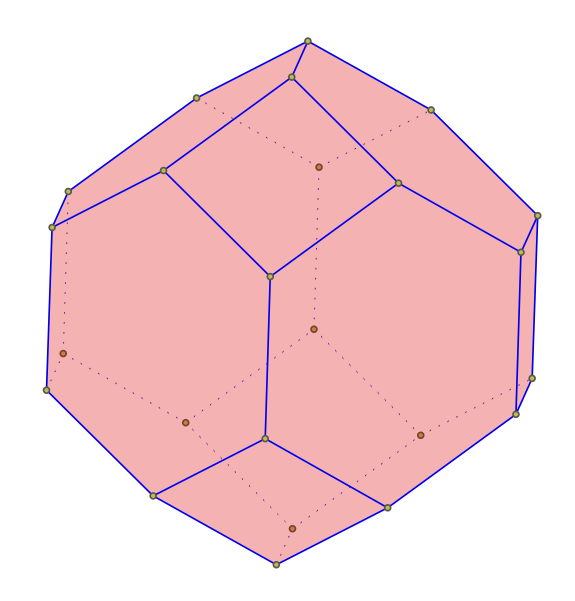
\includegraphics[width=.25\linewidth]{slides_simone/IMAGES/polytope}
    \hspace{1.5cm}
    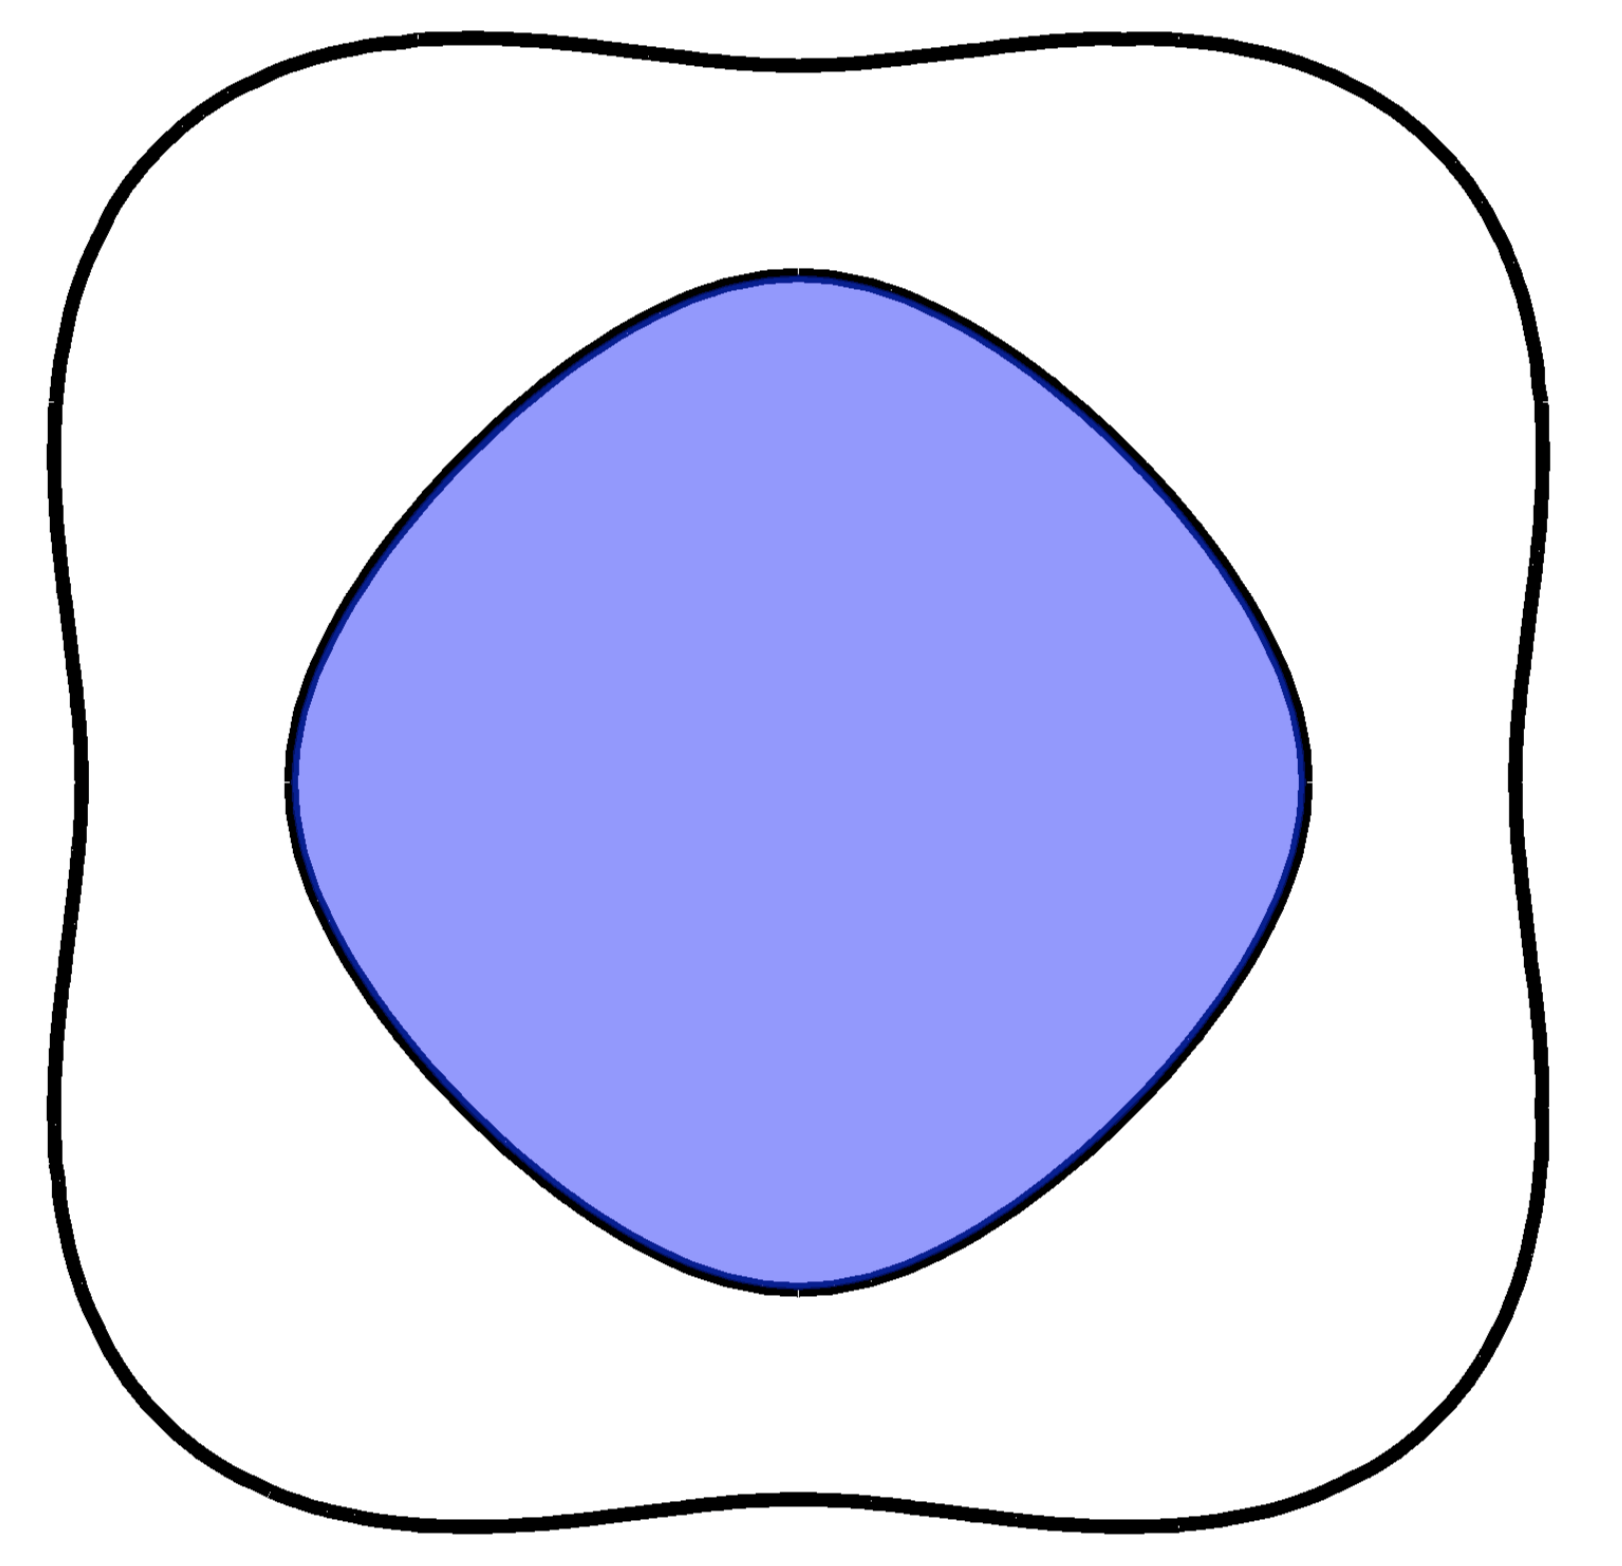
\includegraphics[width=.25\linewidth]{slides_simone/IMAGES/hypcone} \\
    \vspace{0.1cm}
    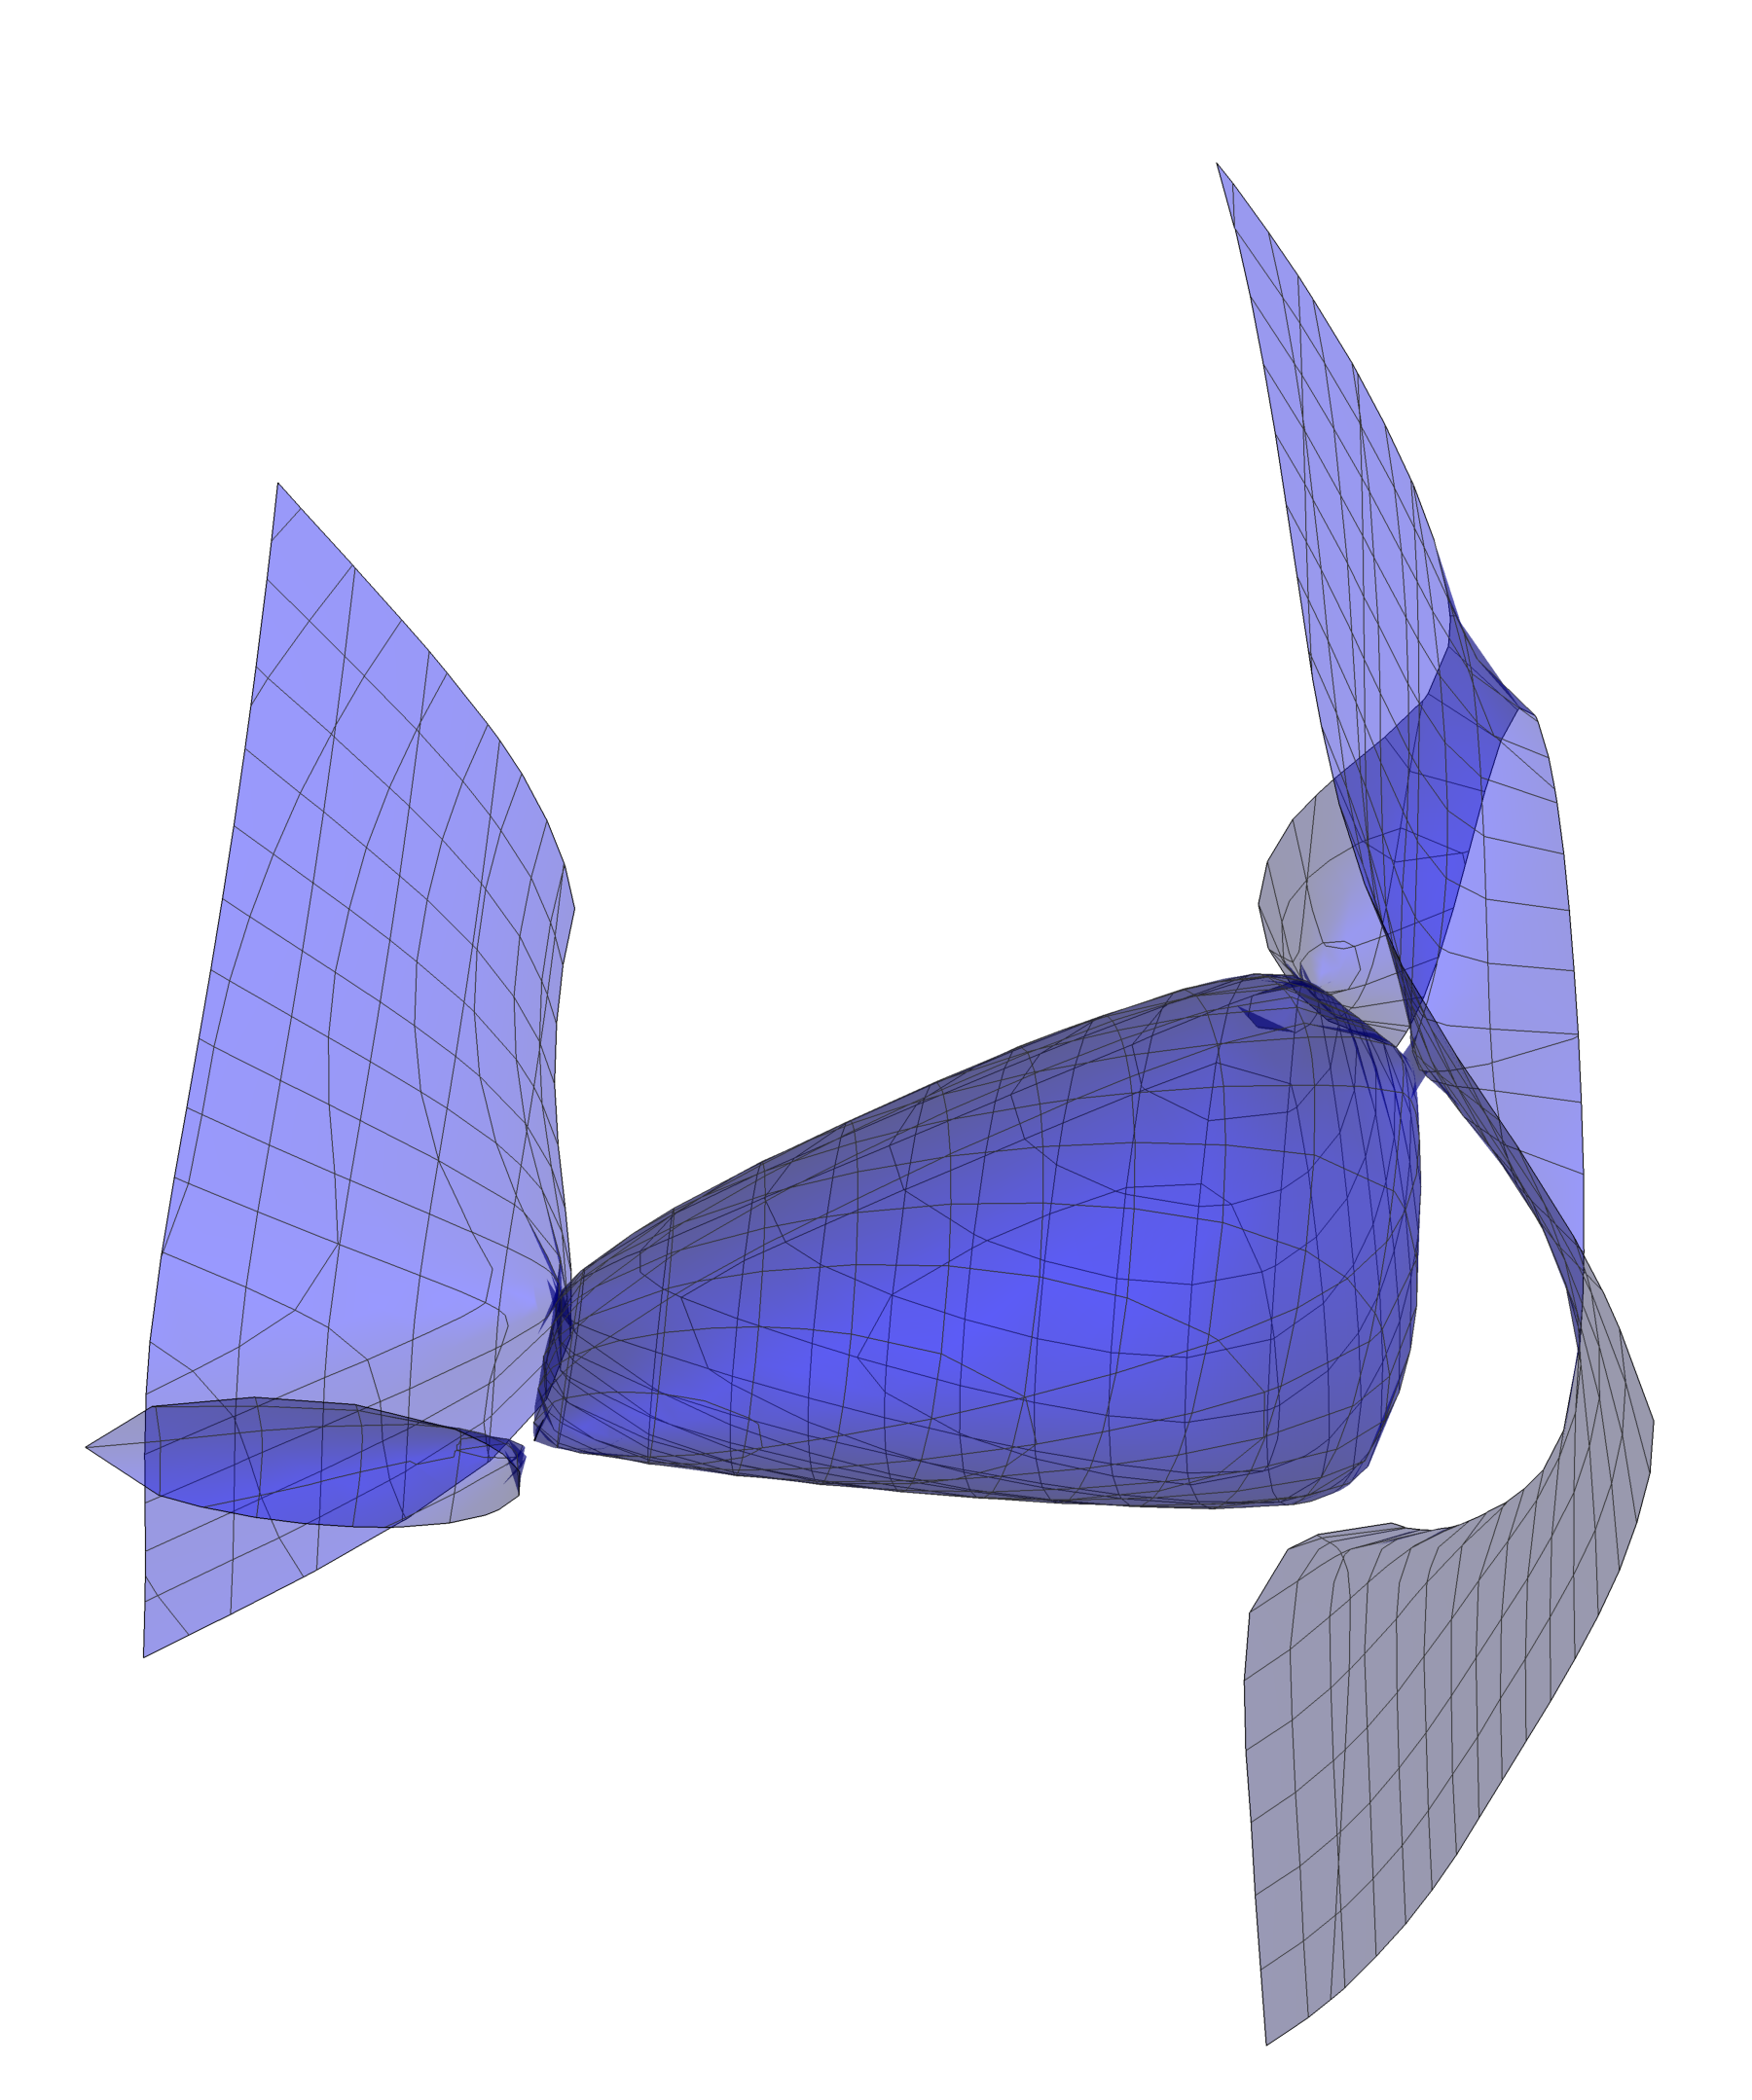
\includegraphics[width=.22\linewidth]{slides_simone/IMAGES/Hyp_Deriv_g}
    \hspace{0.5cm}
    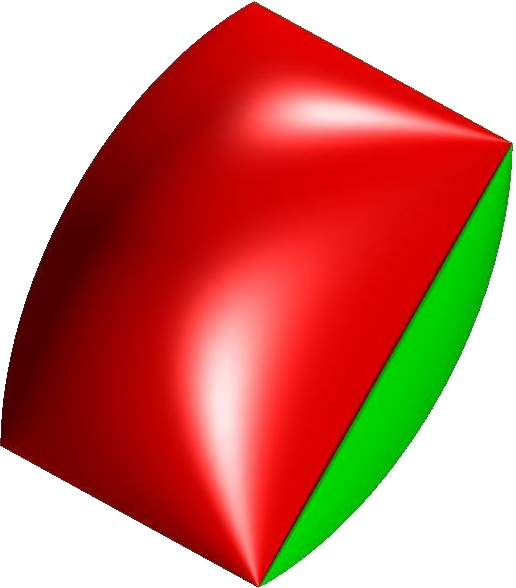
\includegraphics[width=.22\linewidth]{slides_simone/IMAGES/honest_pillow}
    \hspace{0.5cm}
    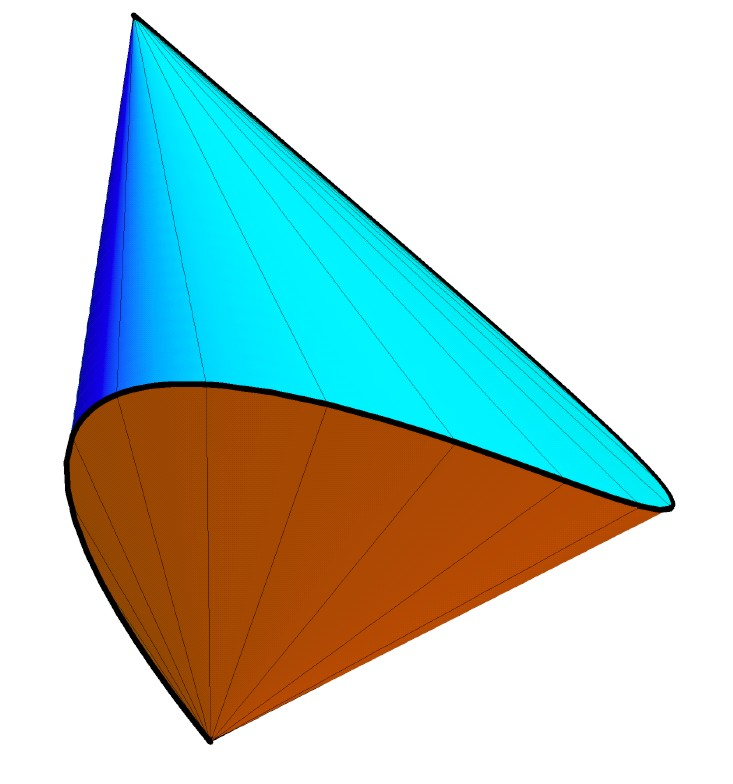
\includegraphics[width=.22\linewidth]{slides_simone/IMAGES/T4}
  \end{figure}
\end{frame}


%%%%%%%%%%%%%%%%%%%%%%%%%%%%%%%%%%%%%%%%%%%%%%%%%%%%%%%%%%%%%%%%%%%%%%%%%%%%%
\begin{frame}
\frametitle{ Motivations and properties}

\vspace{-0.5cm}
\begin{itemize}
\item[] Polyhedra $\rightarrow$ feasible sets of {\color{blue} Linear Programming} ({\color{blue} LP})
  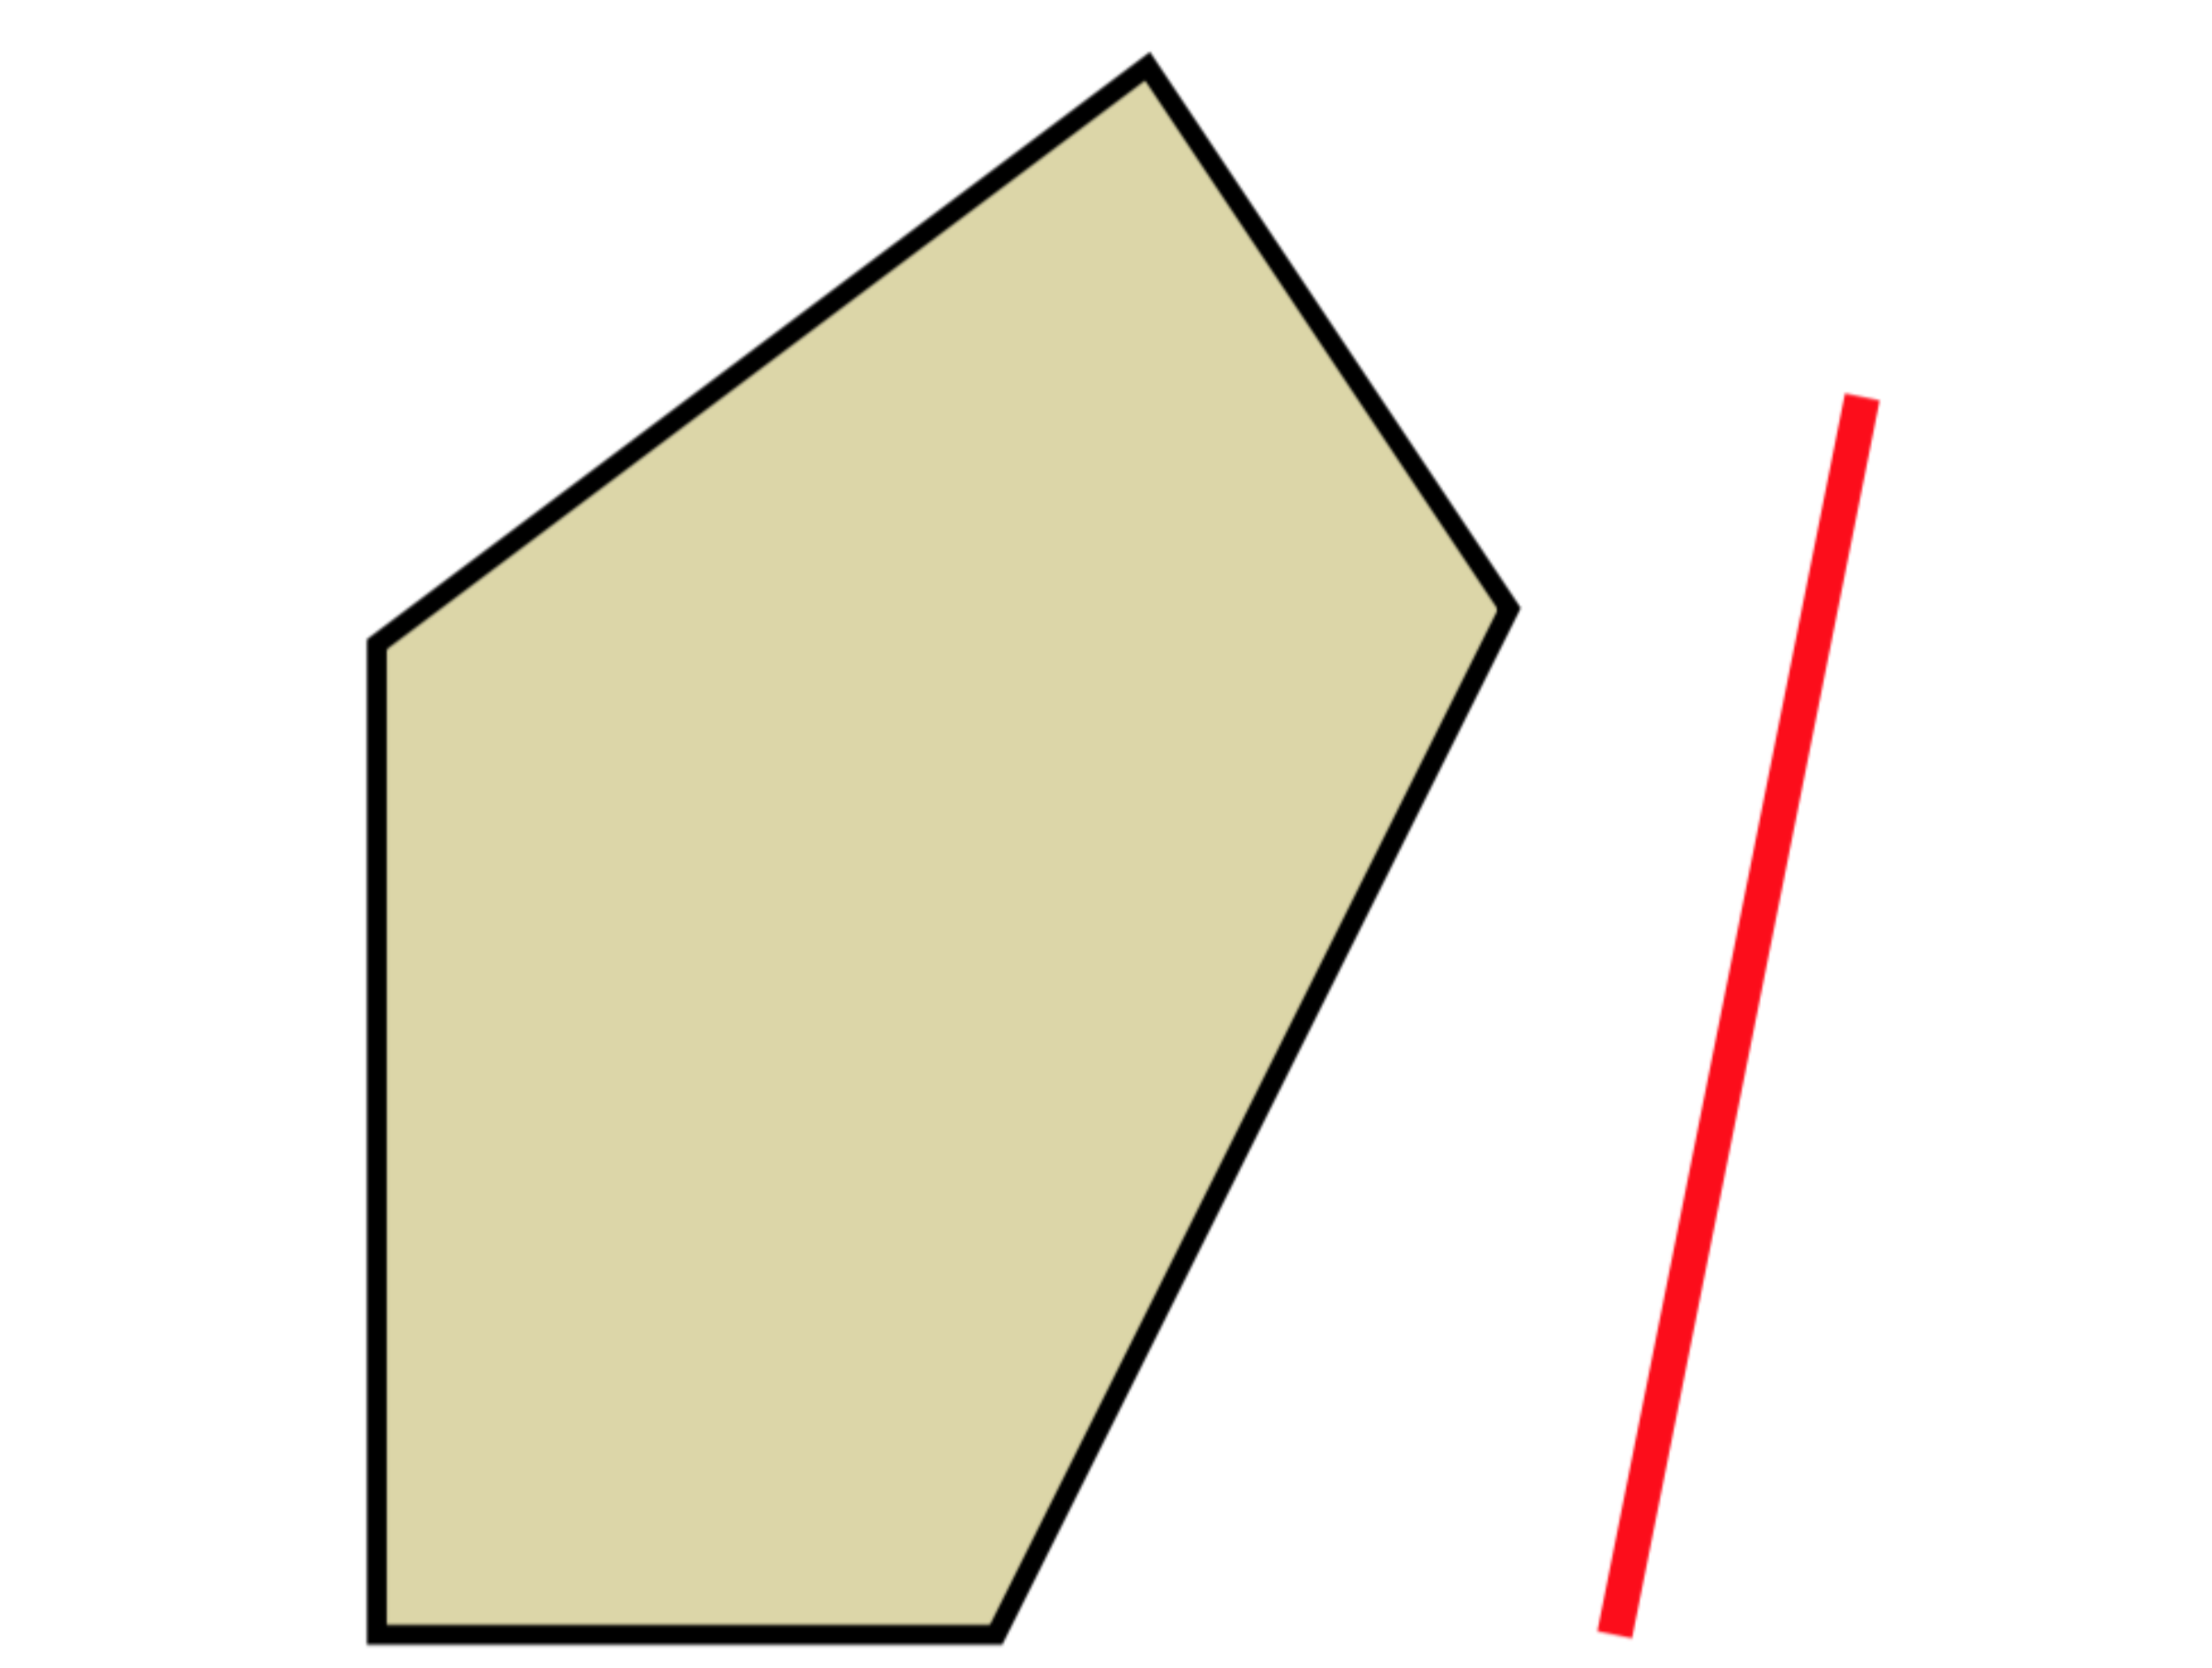
\includegraphics[scale=0.025]{slides_simone/IMAGES/LP_types}
  \vspace{-0.4cm}
\item[] Spectrahedra $\rightarrow$ feasible sets of  {\color{blue} Semidefinite Programming} ({\color{blue} SDP})
  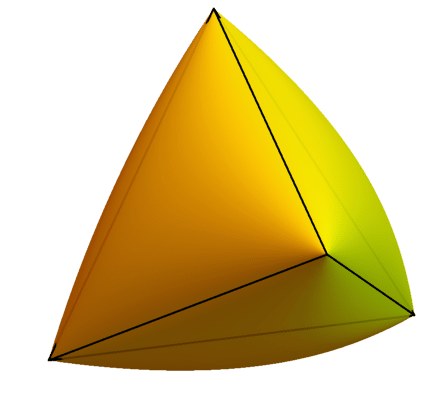
\includegraphics[scale=0.06]{slides_simone/IMAGES/cayley_yellow}
\end{itemize}
\vspace{0.2cm}

\pause

Classical applications from
\begin{itemize}
\item
  {\color{blue} real algebraic geometry} (positive polynomials vs SOS, 17th Hilbert's problem)
\item
  {\color{blue} control theory} (Lyapunov stability)
\item
  {\color{blue} combinatorial optimization} (e.g. SDP relaxation of MAXCUT)
\item
  {\color{blue} polynomial optimization} (moment-SOS relaxation hierarchy)
\end{itemize}

\pause
\vspace{0.2cm}

Several {\bf \color{blue} good properties} besides convex \pause
but spectrahedra/SDP are highly more {\bf \color{red} pathological} than polyhedra/LP:

\begin{itemize}
\item spectrahedra are {\only<5->{\color{olive}\bf}not closed under linear image}
\item solutions only over algebraic extension:
  \scalebox{0.8}{
    $\{\sqrt{2}\} = \left\{x \in \RR :
    \left[\begin{smallmatrix} x & 1 \\ 2 & x\end{smallmatrix}\right] \succeq 0
    \text{ and }
    \left[\begin{smallmatrix} 1 & x \\ x & 2\end{smallmatrix}\right] \succeq 0\right\}$
    }
  %  (points of spectrahedra might not be representable over the defining field)
\item
  in SDP: weak infeasibility, not attainement of inf/sup, etc...
\end{itemize}

\end{frame}


%%%%%%%%%%%%%%%%%%%%%%%%%%%%%%%%%%%%%%%%%%%%%%%%%%%%%%%%%%%%%%%%%%%%%%%%%%%%%
\begin{frame}
\frametitle{Semidefinite representable sets}

The linear projection of a spectrahedron is called a {\color{blue} spectrahedral shadow}:
$$
S = \left\{x \in \RR^n : \exists\, y \in \RR^p, A_0 + \sum_{i=1}^n x_i A_i + \sum_{j=1}^p y_j B_j \succeq 0\right\},
$$
for matrices $A_i,B_j \in \sym^d$. \pause
Spectrahedra and their shadows are in general called {\color{blue} semidefinite representable sets}.
\pause

\begin{figure}
  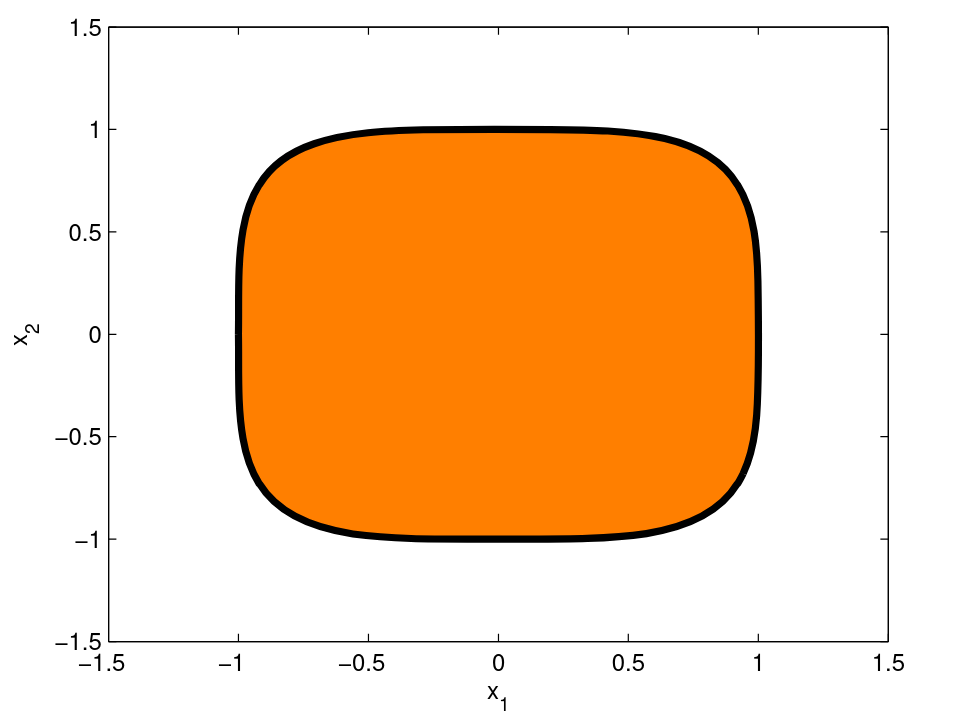
\includegraphics[scale=0.1]{slides_simone/IMAGES/fermat4}
  \centering
  \caption*{\hfill The convex hull of the Fermat's quartic $x^4+y^4=1$ \\
    \hfill is semidefinite representable but not spectrahedral}
\end{figure}
\pause

Not every convex (compact) semialgebraic set is semidefinite representable (Scheiderer, 2018).

\end{frame}



\section{Non-archimedean geometry}

\subsection{Discrete-valuation fields}
\begin{frame}
\frametitle{Setting}

\begin{block}{Discrete-valuation fields}
Let $K$ be a field with:
\begin{itemize}
\item discrete valuation $v_K: \: K \rightarrow \RR \cup \left\lbrace + \infty \right\rbrace$ making it complete,
\item integer ring $O_K$,
\item  residue field $\kappa$,
\item uniformizer $\pi,$ whose valuation generates the additive group $\val (K)$. 
\end{itemize} 
\end{block}
\pause
\begin{expl}
\begin{enumerate}
\item $\QQ_p$, $p$-adic valuation, $\ZZ_p$, $\kappa = \FF_p$, $\pi = p.$
\item $\FF_q((t))$, $t$-adic valuation, $\FF_q[[t]]$, $\kappa = \FF_q$, $\pi = t.$
\item $\QQ((t))$, $t$-adic valuation, $\QQ[[t]]$, $\kappa = \QQ$, $\pi = t.$
\item their finite extensions.
\end{enumerate}
\end{expl}
\pause
Topology somehow in-between discrete and continuous mathematics.
\end{frame}

%pas ordonné
%mais on peut dir eque les >=0 sont les descendants de 0 quelque part...

\subsection{Objects of interest}

\begin{frame}
\frametitle{Non-archimedean balls}

\begin{deftn}[Ball/disks]

\[
D_K(\alpha; \lambda) :=\left\lbrace x \in K : \: v_K(x-\alpha) \geq \lambda \right\rbrace.\]
\end{deftn}



\begin{deftn}[Polydisks]
\[
D_{K^n}(\alpha_1,\dots,\alpha_n; \lambda_1,\dots,\lambda_n) :=\left\lbrace x \in K^n : \: \forall i, \: v_K(x_i-\alpha_i) \geq \lambda_i \right\rbrace.\]
\end{deftn}

\begin{prop}
\begin{itemize}
\item Any point of $D_K(\alpha; \lambda) $  is a center of this disk.
\item If two disks have a non-trivial intersection, then one contains the other. As such, any set of disks as a forest /  tree-like structure for inclusion.
\end{itemize}
\end{prop}



\end{frame}

\begin{frame}
\frametitle{Annuli}

\begin{deftn}[Annulus]
\[\mathcal{C}_{K}(\alpha, a,b) = \{x \in K \,|\, a \le \val(x-\alpha) \le b\},\]
for $x \in K$,  $a \leq b \in \RR.$
\end{deftn}
\begin{center}
\begin{tikzpicture}
\usetikzlibrary{calc}

		\draw[black] (-0.1,0) -- (0.1,0); % Small horizontal line
		\draw[black] (0,-0.1) -- (0,0.1); % Small vertical line
        \node[anchor=south east] at (0,0) {$\alpha$}; % Label "alpha" 
% Annulus
\fill[blue!30, even odd rule]
  (0,0) circle (2)
  (0,0) circle (1);


% Measurement arrows
\draw[<->] (0,0) -- (1,0) node[midway, below] {$a$};
\draw[<->] (0,0) -- (0,-2) node[midway, right] {$b$};
\end{tikzpicture}
\end{center}

\begin{rmk}
Central object in $p$-adic differential equations
or in non-archimedean analytic geometry. 

Used to define series converging on $\mathcal{C}_{K}(\alpha, a,b).$
\end{rmk}

\end{frame}

\begin{frame}
\frametitle{Discoids}

\begin{deftn}
Let $\phi \in K[x]$ be a monic polynomial and let $\lambda \in \Q$. Then
\[
D_K(\phi; \lambda) :=\left\lbrace x \in K : \: v_K(\phi(x)) \geq \lambda \right\rbrace\]
is the \textbf{discoid} with center $\phi$ and radius $\lambda$ over $K$.
\end{deftn}



\begin{rmk}
Discoids play a central role in the family of OM factorization algorithms.

Thanks to recent works with A. Poteaux and M. Weimann, they appear in the clusterization of the roots of polynomials over fields with valuations.
\end{rmk}


\end{frame}

\begin{frame}
\frametitle{Visualizing discoids}

\begin{prop}
If $\phi$ is irreducible over $K$, then $D_{\overline{K}}(\phi; \lambda)$ is the union
of balls of same radius centered around the roots of $\phi.$ The Galois group of $\overline{K}/K$ acts on those balls.
\end{prop}

\begin{center}
\begin{tikzpicture}[scale=0.8]
	    % Mark the origin at (0,0) and label it "O"
		\draw[black] (-0.1,0) -- (0.1,0); % Small horizontal line
		\draw[black] (0,-0.1) -- (0,0.1); % Small vertical line
        \node[anchor=south west] at (0,0) {\textbf{O}}; % Label "O" 

    % Outer circle centered at (0,0) with radius 4
   \draw (0,0) circle (4);

    % Four inner disks with radius 1.5

    \draw (2.5,0) circle (1.5);  % Right
    \draw (-2.5,0) circle (1.5); % Left
    \draw (0,2.5) circle (1.5);  % Top
    \draw (0,-2.5) circle (1.5); % Bottom
    

  
    \draw (.9,2.5) circle (0.6);
    \draw (-0.4,3.26) circle (0.6);
    \draw (-0.4,1.74) circle (0.6);
    
    
    
    
    \draw (3.4,0) circle (0.6); 
\end{tikzpicture}
\end{center}
\end{frame}


\begin{frame}
\frametitle{Visualizing clustering roots in a discrete-valuation field with diskoids}
\begin{center}
\begin{tikzpicture}[scale=0.9]
	    % Mark the origin at (0,0) and label it "O"
		\draw[black] (-0.1,0) -- (0.1,0); % Small horizontal line
		\draw[black] (0,-0.1) -- (0,0.1); % Small vertical line
        \node[anchor=south west] at (0,0) {\textbf{O}}; % Label "O"
    
    \uncover<2->{
    % Outer circle centered at (0,0) with radius 4
   \draw (0,0) circle (4);

    % Four inner disks with radius 1.5

    \draw (2.5,0) circle (1.5);  % Right
    \draw (-2.5,0) circle (1.5); % Left
    \draw (0,2.5) circle (1.5);  % Top
    \draw (0,-2.5) circle (1.5); % Bottom
    

  
    \draw (.9,2.5) circle (0.6);
    \draw (-0.4,3.26) circle (0.6);
    \draw (-0.4,1.74) circle (0.6);
    
    
    
    
    \draw (3.4,0) circle (0.6); }
    
    % Roots
    % In violet
    \fill[violet!80] (1.25,-2.5) circle (0.25);
    \fill[violet!80] (-0.625,-1.41) circle (0.25);
    \fill[violet!80] (-0.625,-3.59) circle (0.25);
    \fill[violet!80] (-1.25,0) circle (0.25);
    \fill[violet!80] (-3.125, 1.09) circle (0.25);
    \fill[violet!80] (-3.125, -1.09) circle (0.25);

    % In green
    \fill[green!70] (1.2,2.5) circle (0.25);
    \fill[green!70] (-0.1,3.26) circle (0.25);
    \fill[green!70] (-0.1,1.74) circle (0.25);

    % In blue    
    \fill[blue!70] (.6,2.5) circle (0.25);
    \fill[blue!70] (-0.70,3.26) circle (0.25);
    \fill[blue!70] (-0.70,1.74) circle (0.25);

    % In red
    \fill[red!80] (3.7,0) circle (0.25);
    \fill[red!80] (3.1,0) circle (0.25);

    % In yellow
    \fill[yellow!80] (2.05, 1.09) circle (0.25);
    \fill[yellow!80] (2.05, -1.09) circle (0.25);
\end{tikzpicture}
\end{center}
\end{frame}





\begin{frame}[fragile, plain]
\frametitle{Clustering roots with discoids and OM algorithm: over $\mathbb{Q}((t))[x]$}


\centering
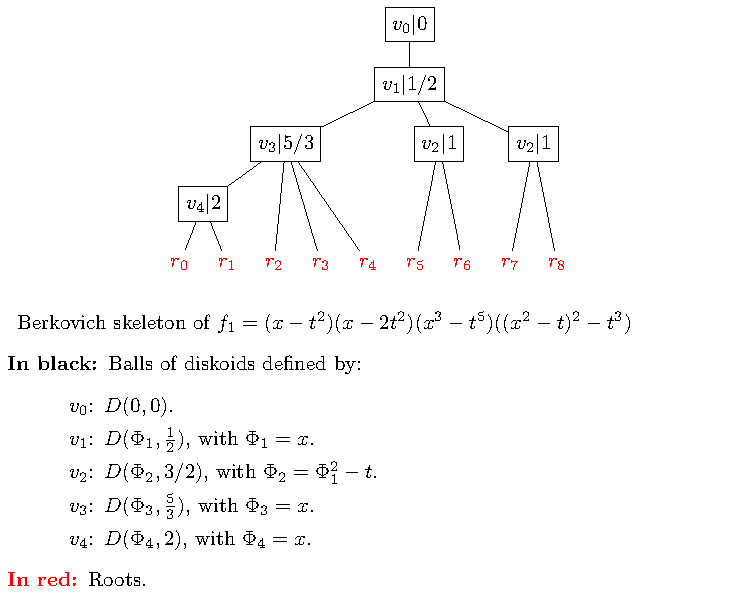
\includegraphics[width=0.8\textwidth]{FBS_f1.pdf}

\end{frame}


\begin{frame}[fragile, plain]
\frametitle{Clustering roots of approximation of polynomials in $\mathbb{Q}((t))[x]$}


\centering
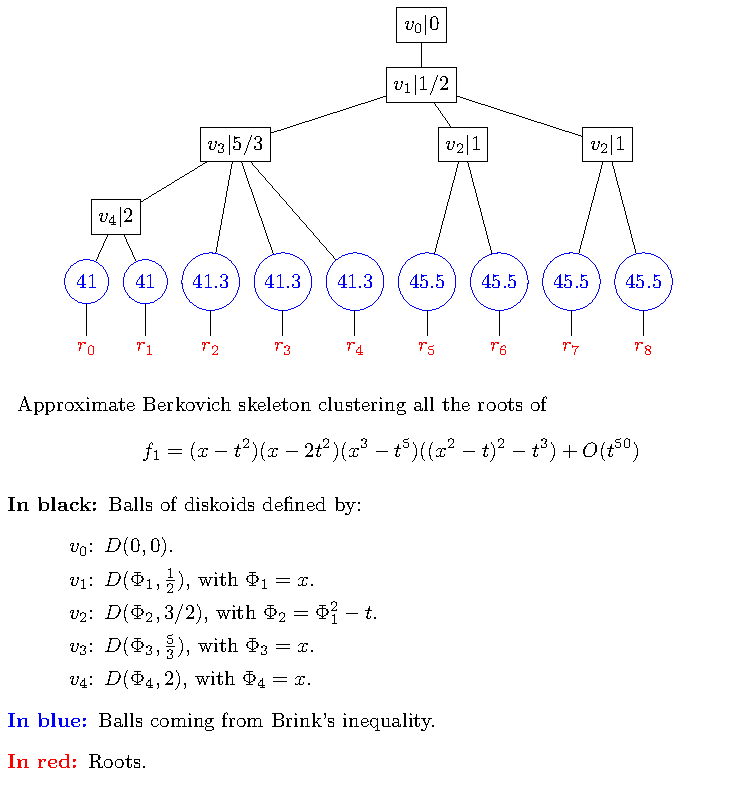
\includegraphics[width=0.62\textwidth]{AFBS_f1.pdf}

\end{frame}

\begin{frame}[fragile, plain]
\frametitle{Clustering roots of approximation of polynomials in $\mathbb{Q}((t))[x]$, multiplicity}


\centering
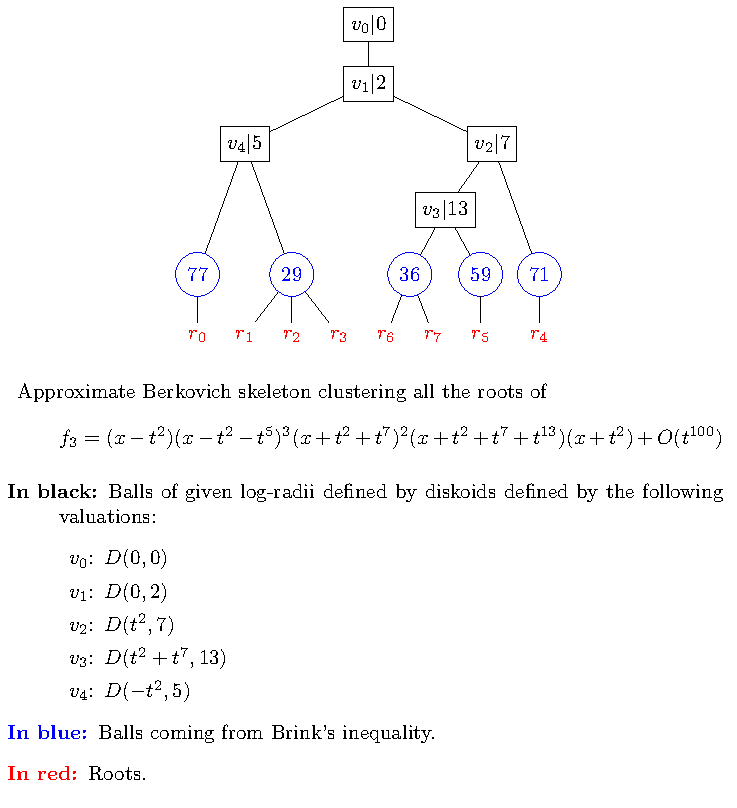
\includegraphics[width=0.60\textwidth]{AFBS_f3.pdf}

\end{frame}

\section{Polyhedron}

\subsection{Definition and first examples}

\begin{frame}
\frametitle{Non-archimedean polyhedron}

\begin{deftn}
  A \emph{polyhedron} is a subset $\PP \subset K^n$ of the form
  \begin{equation}\label{eq_def_polyhedra}
  \PP =
  \left\{
  x \in K^n :
  \begin{array}{ll}
    \val(\ell_i(x)) \geq 0 & i=1,\ldots,d \\
    \val(m_j(x)) = +\infty & j=1,\ldots,e
  \end{array}
    \right\},
  \end{equation}
  for some $\ell_1,\ldots,\ell_d,m_1,\ldots,m_e \in K[x]_1$ (polynomials of degree $1$).
\end{deftn}

This can be written in matrix form:

\begin{equation}
  \PP = \left\lbrace x \in K^n : Ax+v \succeq 0, Bx+w = 0 \right\rbrace,
\end{equation}
for $A \in K^{d \times n}$, $v \in K^d$, $B \in K^{e \times n}$, and
$w \in K^e$ such that $Ax+v = (\ell_1,\ldots,\ell_d)^T$
and $Bx+w = (m_1,\ldots,m_e)^T$.

\begin{expl}
\[ D(c, \alpha) = \left\lbrace x \in K^n : val \left( x-c  \right) \geq \alpha= \right\rbrace= \left\lbrace x \in K^n : val \left( \pi^{-\alpha} (x-c)  \right) \right\rbrace.\]
As such, balls are polyhedron, and similarly for polydisks.
\end{expl}

\end{frame}


\subsection{Stability and applications}

\begin{frame}
\frametitle{Projecting polyhedron}

\begin{thm}[direct image (DI)] \label{theo:DI}
Let $f : K^n \to K^m$ be an affine map and $\PP$ a polyhedron in $K^n.$
Then $f(\PP)$ is a polyhedron in $K^m$.
\end{thm}
\begin{proof}[Idea of proof]

Use the Smith Normal Form of the linear part $f_0$ of $f.$

\[ Mat_B(f_0) = P 
\begin{pmatrix}
\pi^{\alpha_1} & 0 & \cdots & 0 & 0 & \cdots & 0 \\
0 & \pi^{\alpha_2} & \cdots & 0 & 0 & \cdots & 0 \\
\vdots & \vdots & \ddots & \vdots & \vdots & & \vdots \\
0 & 0 & \cdots & \pi^{\alpha_s} & 0 & \cdots & 0 \\
0 & 0 & \cdots & 0 & 0 & \cdots & 0 \\
\vdots & \vdots & & \vdots & \vdots & \ddots & \vdots \\
0 & 0 & \cdots & 0 & 0 & \cdots & 0
\end{pmatrix} Q
\]
with $P, Q \in GL_n(O_K).$

Reduce to the case of: translation, isometry, projection.
\end{proof}

\end{frame}


\begin{frame}
\frametitle{Applications}

\begin{prop}[Characterization of polyhedra]
    A non-empty polyhedron is the image of a polydisc under an affine map.
\end{prop}

\begin{prop} 
   Polyhedra in $K$ are either the empty set or balls, possibly with infinite radius.
\end{prop}


\end{frame}


\section{Spectrahedron}

\subsection{Positive semi-definite matrices}

\newcommand\Mat{Positive semidefinite matrix }
\newcommand\mats{positive semidefinite matrices }
\newcommand\Mats{positive semidefinite matrices }

\begin{frame}
\frametitle{Definition and characterization}
\begin{definition}
  We say that a matrix $M \in K^{d \times d}$ is {positive semidefinite} ($M \succeq 0$)
  if \[\texttt{Spec}_{\overline{K}}(M)  \subset O_{\overline{K}}.\]
  We denote by $K^{d \times d}_+ \subset K^{d\times d}$ the set of positive semidefinite matrices.
\end{definition}

\begin{theorem}
  \label{caracsdp}
  $M \in K^{d\times d}_+$ if and only if $\chi_M \in O_K[T]$.
\end{theorem}
\begin{proof}
Use Newton polygons.
\end{proof}
\begin{cor}
\[ O_K^{d \times d} \subset K^{d \times d}_+.\]
\end{cor}
\end{frame}

\begin{frame}
\frametitle{(Counter)-Example}
\begin{example}
  Let
  $$
  M = \begin{bmatrix} \frac{3}{5}+5 & \frac{4}{5} \\ \frac{4}{5} & -\frac{3}{5} \end{bmatrix} \in \mathbb{Q}_5)^{2 \times 2}.
  $$
  Then \[ \chi_M(T)=T^2-5T-4,\]
	Hence \begin{align*}
	M &\in  (\mathbb{Q}_5)^{2 \times 2}_+ \\
	M & \notin (\mathbb{Z}_5)^{2 \times 2}.
\end{align*}	  
\end{example}
\end{frame}


\subsection{Definitions and first examples}

\begin{frame}
\frametitle{What is a spectrahedron}
\begin{definition}
  \label{def_spectrahedra}
  A \emph{spectrahedron in $K^{d\times d}$} is a set of the form
  $$
  \mathcal{S} = \mathcal{L} \cap K^{d\times d}_+ = \left\{X \in K^{d \times d} :
  \exists \, x \in K^n, X = A_0 + \sum_{i=1}^n x_i A_i, X \succeq 0\right\}
  $$
  where $\mathcal{L} = A_0+\texttt{span}(A_1,\ldots,A_n) \subset K^{d \times d}$ 
  is an affine space, for some
  $A_0,A_1,\ldots,A_n \in K^{d\times d}$.
\end{definition}

\begin{definition}
  \label{def_spectrahedra_Kn}
  A \emph{spectrahedron in $K^n$} is any affine section of a set of the form
  $$
  \mathcal{S}_A = \varphi_A^{-1}(K^{d \times d}_+) = \{x \in K^n : A_0+x_1A_1+\cdots+x_nA_n \succeq 0\}
  $$
  for some $d\in \mathbb{N}$,
  where $\varphi_A : K^n \to \mathcal{L} \subset K^{d \times d}$ is the map
  $\varphi_A(x) = A_0+x_1A_1+\cdots+x_nA_n$, and $\mathcal{L} = A_0+\texttt{span}(A_1,\ldots,A_n)$.
\end{definition}

\end{frame}

\begin{frame}
\frametitle{Polyhedron implies Spectrahedron}

\begin{prop}
  A polyhedron in $K^n$ is a spectrahedron in $K^n$.
\end{prop}
\begin{proof}
  Assume $\PP = L \cap M$ be a polyhedron in $K^n$, with
  $L = \{x \in K^n : \val \ell_i(x) \geq 0, i=1, \ldots, d\}$
  and $M = \{x \in K^n : \val m_j(x) = +\infty, j=1, \ldots, e\}$,
  for some $d, e \in \mathbb{N}$.
  Let $A_0,A_1,\ldots,A_n \in K^{d \times d}$ be such that
  $$
  \varphi_A(x) \coloneq A_0+x_1A_1+\cdots+x_nA_n = \texttt{diag}(\ell_1(x), \ldots, \ell_d(x)).
  $$
  One has $L = \mathcal{S}_A = \varphi_A^{-1}(K^{d \times d}_+)$.
  Since $M \subset K^n$ is affine, then $\PP$ is a spectrahedron in $K^n$.
\end{proof}

\end{frame}

\begin{frame}
\frametitle{Some spectrahedron are not polyhedron}
\begin{example}
  The following spectrahedron is not a polyhedron:
  \[
  \mathcal{S} = \left\{x \in K : \begin{bmatrix} 0 & x + \pi^{-1} \\ x & 0 \end{bmatrix} \succeq 0\right\}.
  \] 
\end{example}
\begin{proof}
  By characterization of positive semi-definite matrices, one has $\mathcal{S} = \{x \in K : \val(x(x + \pi^{-1})) \geq 0\} =
  \{x \in K: \val x \ge 1\} \cup \{x \in K: \val (x - \pi^{-1}) \ge 1\}$ which is not a ball in $K$.
  Therefore, $\mathcal{S}$ is not a polyhedron.
\end{proof}

\end{frame}


\begin{frame}
\frametitle{Spectrahedron in $K$}

\begin{prop}
Spectrahedra of $K$ are diskoids. 
\end{prop}
\begin{proof}
If $S$ is a spectrahedra of $K$ not reduced to a point, then
\begin{align*}
S &= \{x \in K : A_0+x A_1 \succeq 0\} \\
  &= \cap_{i=0}^{d-1} \{x \in K : \val(a_i(x)) \geq 0\}\\
\end{align*}
for some integer $d$, matrices $A_0$ and $A_1$ in $K^{d \times d}$,
The intersection
of two diskoids is either empty or a diskoid.
Consequently, spectrahedra of $K$ are diskoids.
\end{proof}
\end{frame}


\subsection{Polyannuli}

\begin{frame}
\frametitle{Spectrahedral shadows}
\begin{deftn}[Semidefinite-representable set]\label{def_semi_def_rep_set}
  A set $\mathcal{R} \subset K^n$ is called
  \emph{semide\-fi\-nite-re\-pre\-sen\-ta\-ble (SDR)} if there exist $m,d \in \NN$
	and a spectrahedron $\mathcal{S} \subset K^{n+m}$
	such that \[\mathcal{R} = \texttt{proj}_{\leq n}(\mathcal{S})\]
	with $  \texttt{proj}_{\leq n}: \: K^{n+m} \rightarrow K^n$ the projection on the first $n$ components.
\end{deftn}

If $m\geq 1$, we can also write that $\mathcal{R}$ is a spectrahedral shadow.
\end{frame}


\begin{frame}
\frametitle{Annuli and shadows}

\begin{thm}
Annuli in $K$ such as $\mathcal{C}_{K}(0, a,b) = \{x \in K \,|\, a \le \val(x) \le b\}$ are spectrahedral shadows.
\end{thm}
\begin{proof} \vspace{-.5cm}
  $$
  M(x,y) \coloneq \left(
  \begin{bmatrix}
  	\pi^{-a} x & 0 & 0 & 0 \\
  	0 & \pi^{b} y & 0 & 0 \\
    0 & 0 & \pi^{-1} & -\pi^{-1} x  \\
    0 & 0 & \pi^{-1} y & - \pi^{-1} \\
  \end{bmatrix}\right) \succeq 0.
  $$
  Then $M \succeq 0$ if and only if $(x,y)$ is a solution of the system
  of inequalities:
  \begin{equation}
    \label{eq:annulussyst}
    \begin{cases}
      \val(\pi^{-a} x) \ge 0 \\
  \val(\pi^{b} y) \ge 0\\
  \val(\pi^{-1}- \pi^{-1}) = +\infty \ge 0\\
  \val(\pi^{-2}\left( xy-1 \right))  \ge 0 
\end{cases}
\iff	
\begin{cases} 
  \val\left(x\right)\ge a\\
  \val\left(y\right)\ge -b\\
  \val\left(xy-1 \right) \ge 2
\end{cases}
\end{equation} 

  Thus $\val\left(x\right)+\val\left(y\right)=\val\left(xy\right) = \val\left(-1\right) =0$.
  Therefore $\val\left(x\right)=-\val\left(y\right)\le -(-b) = b$ and $x \in \mathcal{C}_K(0,a,b)$. 
The converse is clear and $\mathcal{C}_K(0,a,b)$ is the proj. of the spectrahedra defined by $M.$
\end{proof}

\end{frame}

\begin{frame}
\frametitle{Annuli and spectrahedron}

\begin{thm}
If the residue field of $K$ is infinite, no (non-trivial) annulus of $K$ can be a spectrahedron of $K.$
\end{thm}
\begin{proof}
Spectrahedron of $K$ are diskoids and thus are finite union of balls.

If the residue field of $K$ is infinite, no annulus
can be finite union of balls.

For example: 
\[ \{x \in K \,|\,  \val(x) =0\}=\amalg_{l \in \kappa} B(b_l, \vert \pi \vert)\] for some representatives $b_l \in O_K$ of the classes of $O_K / \pi O_K = \kappa.$
It thus can not be covered by a finite amount of balls of radius $\vert \pi \vert$
and if one take any ball of radius $1$ centered at a point of the sphere, then one gets the whole
$B(0,1).$

One can generalize this argument to annuli.
\end{proof}
\end{frame}


\section*{Conclusion}

\begin{frame}
\frametitle{Conclusion}
\begin{block}{Summary}
\begin{itemize}
\item Definition of polyhedron and spectrahedron over $K$. \pause
\item Connection with some basic objects of non-archimedean geometry: balls, annuli and diskoids. \pause
\item Also in the article: solving problems of linear programming in $K$. \pause
\end{itemize}
\end{block}
\begin{block}{Future works}
\begin{itemize}
\item Can we decide if a spectrahedron is non-empty? \pause
\item Can we give an explicit representation? \pause
\end{itemize}
\end{block}
\end{frame}

\begin{frame}
\frametitle{Thank you for your attention}
\vspace{-.2cm}
\begin{block}{Thank you} 
\vspace{-.25cm}
\begin{tikzpicture}

\draw[dotted] (1.5,-1.5) -- (1.5,5.2);
\draw[dotted] (-4,1.5) -- (6.9,1.5);



\draw[red, thick] (-2,3) circle (.75cm);
\node[left,red] at (-2.75,2.7) {$x+B$};


\draw[->, >=latex] (-1,2.7) to[bend right] (3,2.7) ;
\node at (1,1.7) {$f$};

\node[left,red] at (-3,0) {$B$};
\draw[red,thick] (-2,0) circle (.75cm);



%\node[right] at (4.7,3) {$f(x)$};
\draw (4.1,3.4) -- (4.1,3.2);
\draw (4.0,3.3) -- (4.2,3.3);


\draw[->, >=latex] (-1,0.1) to[bend left] (3,0.1) ;
\node at (1,1.1) {$f'(x)$};


\draw[red,thick] (4,3) ellipse (.5cm and 1.25cm);






\node[right,red] at (4.45,2.5) {$f(x)+f'(x)\cdot B$};


\node[right,red] at (4.7,0) {$f'(x) \cdot B$};
\draw[red,thick] (4,0) ellipse (.5cm and 1.25cm);



\draw[->, >=latex, brown] (-1,3.3) to[bend left] (3,3.3) ;
\node[brown, thick] at (1,4.1) {$\widetilde{f}$};


%\draw[brown, thick] (3.2,4.5)  rectangle  (5, 1.6);


\draw[brown, thick] (-2.15,3.35)  rectangle  (-1.85, 3.05);
\node[left, brown] at (-2,3) {$x$};
\draw[brown] (-2,3.3) -- (-2,3.1);
\draw[brown] (-2.1,3.2) -- (-1.9,3.2);




\draw[brown, thick] (3.6,3.5)  rectangle  (4.4, 2.8);

\draw[dotted] (-4,4.5) -- (6.9,4.5);





\node[brown] at (-2,4.8) {$x+O(p^{N'})$};

\node[ brown] at (2.8,4.8) {$y+O(p^{M'}) \subset $};
\node[ red] at (5,4.8) {$f(x)+O(p^{N})$};
\end{tikzpicture}
\end{block}
\end{frame}



\begin{frame}
\frametitle{References}
\begin{small}
\begin{block}{OM algorithms and diskoids}
\begin{itemize}
\item \textbf{PVW2025}, \textit{On OM algorithms and Cluster Pictures}, A. Poteaux, T. Vaccon, M. Weimann, 2025.
\item \textbf{PVW2026}, \textit{On OM algorithms and Cluster Pictures II: handling small precision}, A. Poteaux, T. Vaccon, M. Weimann, 2026.
\end{itemize}
\end{block}
\begin{block}{Polyhedron and spectrahedron over valued fields}
\begin{itemize}
\item \textbf{CNV2025}: \textit{On semidefinite-representable sets over valued fields}, C. Cornou, S. Naldi, T. Vaccon, 2026
\end{itemize}
\end{block}
\begin{block}{A tropical approach to spectrahedra in a non-archimedean context (unrelated)}
\begin{itemize}
\item \textbf{AGS2020}: \textit{Tropical Spectrahedra}, X. Allamigeon, S. Gaubert, M. Skomra, 2020
\end{itemize}
\end{block}
\end{small}
\end{frame}


\end{document}
